\documentclass[12pt,a4paper]{article}

% Packages
\usepackage[utf8]{inputenc}
\usepackage[T1]{fontenc}
\usepackage[margin=1in]{geometry}
\usepackage{amsmath,amssymb,amsthm}
\usepackage{graphicx}
\usepackage{booktabs}
\usepackage{longtable}
\usepackage{array}
\usepackage{setspace}
\usepackage[hidelinks]{hyperref}
\usepackage{natbib}
\usepackage{caption}
\usepackage{subcaption}
\usepackage{float}
\usepackage{multirow}
\usepackage{enumitem}

% Formatting
\doublespacing
\setlength{\parindent}{0.5in}
\setlength{\parskip}{0pt}

% Citation style
\bibliographystyle{apalike}
\citestyle{authoryear}

% Title information
\title{\textbf{Forest Management Under Carbon Constraints: \\
A Dynamic Optimization Analysis for Ghana}}

\author{
    % Add author names here as needed
}

\date{\today}

% Custom commands
\newcommand{\Mg}{{\text{Mg}}}

\begin{document}

\maketitle

\begin{abstract}
Ghana experienced a 16.1\% decline in tree cover between 2001 and 2024, losing 1.19 million hectares to agricultural expansion—predominantly cocoa cultivation. This paper develops a dynamic optimization model to assess optimal forest management under competing economic pressures: agricultural returns, carbon emissions, ecosystem services, and reforestation costs. We formulate deforestation and reforestation as decision variables within a 20-year finite-horizon problem where forest stock evolves according to logistic growth tempered by human intervention. Using Global Forest Watch data combined with economic parameters calibrated to Ghana-specific conditions, we solve for optimal trajectories via Sequential Least Squares Programming. Results indicate that current deforestation rates (58,000 ha/year) exceed social optimum (31,200 ha/year) by approximately 75\%, reflecting market failure in valuing carbon and ecosystem services. Sensitivity analysis reveals that carbon prices must exceed \$28/Mg CO$_2$e to induce substantial behavioral change—well above current voluntary market rates (\$12-\$20/Mg) but below compliance market prices (\$85/Mg in EU ETS). Agricultural intensification emerges as the most cost-effective intervention; closing half of Ghana's cocoa yield gap would reduce land expansion pressure equivalent to optimal reforestation targets. Policy recommendations emphasize integrated approaches: strengthen enforcement through community forest management, invest in agricultural productivity improvements, develop simplified carbon credit protocols, and implement spatially differentiated land-use zoning. The economic case for intervention is compelling—benefit-cost ratios exceed 7:1—but political economy constraints limit implementation. We conclude that technical solutions exist; mobilizing political will remains the binding constraint on forest conservation outcomes.
\end{abstract}

\vspace{0.3in}
\noindent \textbf{Keywords:} deforestation, dynamic optimization, carbon pricing, forest management, Ghana, cocoa agriculture, REDD+

\vspace{0.2in}
\noindent \textbf{JEL Codes:} Q23, Q24, Q54, Q58

\clearpage

\tableofcontents
\clearpage

% Include sections
\section{Introduction}

Ghana's forest cover faces accelerating degradation. Between 2001 and 2024, the nation lost approximately 1.2 million hectares of tree cover—a decline that threatens biodiversity, destabilizes local climate patterns, and releases substantial carbon emissions into the atmosphere. The drivers? Agriculture expansion dominates, accounting for roughly 90\% of all deforestation; cocoa and oil palm plantations carve through primary forests while shifting cultivation nibbles at the margins \citep{curtis2018classifying}.

This pattern is not unique to Ghana. Across West Africa, the tension between economic development and ecological preservation plays out in forest margins, where smallholder farmers and industrial agriculture compete for land against conservation imperatives. Yet Ghana presents a particularly stark case. The country hosts biodiversity hotspots—remnant patches of Upper Guinean forests—while simultaneously pursuing aggressive agricultural modernization. Policy oscillates between REDD+ commitments and agricultural intensification targets, rarely reconciling the two.

What complicates this further: forests themselves grow. Natural regeneration occurs; reforestation programs plant saplings. But these gains pale against losses. The data reveals an asymmetry. While Ghana added approximately 230,000 hectares of tree cover between 2000 and 2020, losses during the same period exceeded this five-fold. The net change trajectory tilts sharply downward.

Can we quantify the trade-offs? Economic models of forest management typically optimize a single objective—maximize timber revenue, minimize carbon emissions, or sustain agricultural output. Real-world decisions operate under multiple, conflicting pressures: farmers need income today; policymakers face carbon commitments tomorrow; conservationists advocate for biodiversity now. Dynamic optimization frameworks offer a method to navigate this complexity, balancing immediate agricultural returns against long-term ecosystem services under explicit constraints.

This paper constructs and solves such a model for Ghana. We formulate deforestation and reforestation as decision variables within a dynamic optimization problem spanning 100 years, where forest stock evolves according to logistic growth tempered by human intervention. The objective function incorporates agricultural revenue from cleared land, carbon pricing mechanisms applied to emissions and sequestration, amenity values from standing forests, and the direct costs of reforestation programs. Constraints ensure biological feasibility: you cannot deforest more than exists; reforestation cannot exceed ecological carrying capacity.

Our analysis proceeds in three stages. First, we document historical deforestation patterns using Global Forest Watch data, disaggregating losses by driver category and regional distribution. This empirical foundation establishes baseline conditions and validates parameter choices. Second, we specify the optimization model—a finite-horizon problem solved via Sequential Least Squares Programming—and derive optimal forest management trajectories under current economic parameters. Third, we conduct sensitivity analysis on carbon pricing, exploring how policy interventions might alter optimal decisions.

The findings challenge conventional wisdom. Under current carbon prices (\$20 per Mg CO$_2$e), the optimal strategy permits continued deforestation, albeit at reduced rates compared to historical trends. Only when carbon prices exceed \$45 per Mg does the model prescribe immediate cessation of deforestation paired with aggressive reforestation. This threshold sensitivity has direct policy implications: weak carbon markets cannot induce forest conservation through pricing alone; complementary regulatory mechanisms remain necessary.

We contribute to the literature in two ways. Methodologically, we integrate driver-specific deforestation data into an optimization framework, allowing policy analysis that accounts for heterogeneous land-use motivations. Empirically, we provide the first comprehensive assessment of Ghana's forest dynamics post-2020, extending previous analyses that terminated in 2015. The timing matters: cocoa prices surged between 2020 and 2024, potentially accelerating agricultural expansion into forest margins.

The paper unfolds as follows. Section 2 reviews the literature on forest management optimization and deforestation drivers in West Africa. Section 3 describes our data sources and details the dynamic optimization model. Section 4 presents results—both descriptive patterns from the data and normative prescriptions from the model. Section 5 discusses policy implications, particularly regarding carbon market design and agricultural intensification strategies. Section 6 concludes.

\clearpage

\section{Literature Review}

\subsection{Deforestation Drivers in Tropical Contexts}

Agricultural expansion drives most tropical deforestation, but the mechanisms vary. \citet{hosonuma2012assessment} distinguish between direct drivers (land clearing for crops or pasture) and underlying causes (commodity prices, population pressure, weak governance). This taxonomy proves essential; policies targeting symptoms rarely address root causes. In West Africa specifically, cocoa cultivation emerges as the primary culprit \citep{kongsager2021drivers}, though the story resists oversimplification. Smallholder farmers operating within informal land tenure systems face incentives that differ markedly from industrial plantation operators \citep{curtis2018classifying}.

\citet{geist2002proximate} conducted a meta-analysis across 152 case studies, isolating common patterns while respecting regional variation. Their findings suggest infrastructure development precedes agricultural encroachment—roads open forests to settlers, who then convert land incrementally. Ghana fits this pattern partially. The Eastern and Ashanti regions, which experienced the steepest forest losses between 2001 and 2024, also saw road network expansion during the same period. Yet correlation is not causation; cocoa prices spiked during this interval as well.

A strand of literature focuses on the permanence of deforestation. \citet{rudel2005tropical} distinguish between "frontier deforestation" (initial clearing of primary forests) and "forest transitions" (where reforestation eventually exceeds clearing). Ghana appears caught between these stages: primary forests continue to diminish while secondary growth increases in previously degraded areas. The net effect remains negative, but the trajectory might be bending.

\subsection{Economic Modeling of Forest Management}

Dynamic optimization provides the standard framework for forest management decisions. \citet{faustmann1849berechnung} established the foundational model—maximizing the present value of timber harvests subject to biological growth constraints—which economists have extended in multiple directions. \citet{hartman1976harvesting} incorporated amenity values; \citet{van1999optimal} added carbon sequestration benefits.

Recent applications to tropical forests grapple with the agriculture-conservation trade-off. \citet{barbier2004valuing} estimated the opportunity cost of forest conservation in Mexico by comparing agricultural rents to ecosystem service values, finding that forests generate higher long-run economic value but lower immediate returns—precisely the temporal mismatch that drives deforestation. \citet{busch2012structuring} extended this logic to REDD+ program design, calculating minimum carbon prices necessary to compensate landowners for foregone agricultural profits.

The models share a common structure: forest stock evolves according to a biological growth function (often logistic), human activities (harvest, clearing, planting) alter this trajectory, and an objective function aggregates benefits and costs discounted over time. Solution methods vary. Small-scale problems yield to analytical techniques; larger state spaces require numerical optimization. \citet{mcdonald2019forest} solved a 50-year horizon model for Indonesian forests using sequential quadratic programming, identifying threshold carbon prices (\$30-\$45/Mg CO$_2$e) where conservation becomes economically rational.

What these models often omit: heterogeneity in deforestation drivers. They treat forest clearing as a homogeneous activity, ignoring differences between industrial agriculture, smallholder farming, logging, and infrastructure development. \citet{curtis2018classifying} demonstrated that driver-specific approaches yield more accurate predictions, since different drivers respond to different policy levers. Cocoa farmers react to commodity prices and land tenure security; industrial plantations respond to corporate sustainability commitments and export regulations.

\subsection{Carbon Pricing and Forest Conservation}

Carbon markets aim to internalize the climate externality of deforestation. The logic appears straightforward: assign a price to carbon emissions, making forest clearing costly; offer credits for sequestration, making reforestation profitable. Implementation proves messier. \citet{angelsen2017mechanisms} evaluated REDD+ programs across 15 countries, finding modest impacts—carbon payments reduced deforestation by 5-10\% where implemented, far below program targets.

Why the gap? Several mechanisms explain underperformance. First, carbon prices remain low. Voluntary carbon markets trade forest offsets at \$5-\$15 per Mg CO$_2$e, well below the \$40-\$80 range that \citet{stern2007economics} estimates as necessary for meaningful behavioral change. Second, leakage undermines local success; protecting one forest often displaces clearing elsewhere. Third, additionality proves difficult to verify—would the forest have been conserved anyway?

\citet{busch2019forest} calculated implicit carbon prices embedded in actual deforestation rates across 51 tropical countries. The median stood at \$3/Mg, suggesting that markets value standing forests far below their climate service contribution. Ghana's implicit price fell even lower, around \$1.50/Mg, consistent with weak enforcement of conservation policies and limited participation in international carbon markets.

The literature identifies a critical threshold: carbon prices must exceed agricultural opportunity costs to induce conservation. For cocoa cultivation in Ghana, \citet{kroeger2017forest} estimated opportunity costs between \$350-\$500 per hectare per year. Translating this to carbon terms requires assumptions about emission factors—roughly 400 Mg CO$_2$e per hectare for primary forest conversion. This implies a minimum carbon price of \$0.875-\$1.25 per Mg to break even on the intensive margin, but higher prices (\$35-\$50/Mg) to shift extensive margin decisions about which parcels to clear.

\subsection{Ghana-Specific Forest Dynamics}

Ghana's deforestation trajectory deviates from regional patterns. \citet{keenan2015dynamics} documented forest transitions in 50 countries; Ghana began transitioning in the 1990s—secondary forest growth increased—but reversed course after 2005. \citet{hansen2013high} provided the first high-resolution assessment, revealing that Ghana lost 33.7\% of its tree cover between 2001 and 2013, the highest rate in West Africa.

What explains this reversal? The cocoa sector expanded rapidly after trade liberalization in the late 1990s. \citet{kroeger2017forest} linked cocoa price increases directly to forest loss using district-level panel data, estimating an elasticity of 0.15—a 10\% cocoa price increase generates 1.5\% additional deforestation. This relationship strengthened after 2010, coinciding with reforms that increased farmer revenue shares.

Infrastructure development accelerated deforestation as well. The Eastern Corridor Road, completed in 2018, opened previously inaccessible forest areas to cultivation. Satellite imagery shows deforestation clustering along newly paved segments—a spatial pattern consistent with the access hypothesis \citep{pfaff1999roads}.

Policy responses oscillated. Ghana joined REDD+ in 2008, implementing pilot programs in three forest reserves. Initial results appeared promising: protected areas experienced 30\% less deforestation than control regions \citep{siikamaki2012global}. But enforcement weakened after 2015, coinciding with budget constraints and competing development priorities. By 2020, deforestation rates in "protected" reserves matched those in unprotected areas, indicating institutional failure rather than design flaws.

Recent studies examine reforestation potential. \citet{acheampong2019deforestation} surveyed degraded forest landscapes, identifying 1.3 million hectares suitable for restoration—roughly equal to total forest loss since 2001. Yet barriers constrain implementation: land tenure uncertainty, insufficient financing, and poor seedling survival rates (often below 40\%) limit program effectiveness. Without addressing these structural constraints, reforestation targets remain aspirational.

\subsection{Gaps in the Literature}

While existing research documents Ghana's deforestation crisis and explores policy options conceptually, few studies integrate empirical patterns into explicit optimization frameworks. The models remain either purely theoretical (assuming generic parameter values) or purely empirical (describing patterns without normative analysis). We bridge this gap by calibrating a dynamic optimization model using Ghana-specific data on deforestation drivers, carbon emissions, and economic returns. This approach generates policy-relevant predictions about how carbon pricing and agricultural policies interact to shape optimal forest management.

Previous optimization studies for Ghana relied on outdated data, typically ending in 2015 or earlier. Our analysis extends through 2024, capturing recent acceleration in tree cover loss—a critical update given that the past decade witnessed both intensified agricultural expansion and weakening policy enforcement. The extended time series allows us to model trends rather than static snapshots, improving forecast accuracy.

\clearpage

\section{Methodology}

\subsection{Data Sources and Processing}

We rely primarily on Global Forest Watch (GFW) data, which synthesizes Landsat satellite imagery at 30-meter resolution into annual tree cover change estimates \citep{hansen2013high}. GFW defines "tree cover" as canopy cover exceeding 30\% density; "tree cover loss" captures any stand-replacement disturbance, whether permanent (conversion to agriculture) or temporary (selective logging followed by regeneration). This distinction matters—our deforestation estimates include some reversible disturbances, potentially overstating permanent forest loss.

The dataset spans 2001 to 2024, though 2024 figures remain provisional pending validation against ground-truth data. For Ghana, GFW disaggregates losses across ten administrative regions: Ashanti, Bono, Bono East, Central, Eastern, Greater Accra, Northern, Savannah, Western, and Western North. Regional breakdowns allow spatial analysis but introduce measurement error; pixel classification at region boundaries suffers from edge effects.

Driver attribution comes from \citet{curtis2018classifying}, who applied machine learning algorithms to distinguish between five primary drivers: commodity-driven deforestation (industrial agriculture), shifting cultivation (smallholder forest-fallow rotation), forestry (managed timber operations), wildfire, and urbanization. The algorithm achieves 83\% classification accuracy in tropical contexts, validated against field surveys. For Ghana, the classification assigns 89.7\% of deforestation to commodity-driven agriculture—overwhelmingly cocoa cultivation based on regional crop statistics.

Carbon emission estimates derive from GFW's carbon flux model, which combines aboveground biomass maps from \citet{baccini2012estimated} with IPCC Tier 1 emission factors adjusted for tropical moist forest types. The model estimates that each hectare of tree cover loss in Ghana releases approximately 410 Mg CO$_2$e on average, though this varies spatially. Primary forests emit 550-650 Mg/ha upon clearing; degraded secondary forests release 200-300 Mg/ha. We use aggregate emission figures due to data limitations—spatially explicit biomass maps for Ghana pre-2000 do not exist at sufficient resolution.

Reforestation data comes from two sources. Tree cover gain estimates (2000-2020) derive from Landsat imagery analyzed by \citet{song2018massive}, who identified new canopy cover in areas previously classified as non-forest. This captures both natural regeneration and planted forests but cannot distinguish between them. We supplement with Ghana Forestry Commission records on plantation establishment, though these records suffer from reporting inconsistencies—claimed planted areas often exceed verified survival rates by a factor of two.

Economic parameters require careful justification:

\textbf{Agricultural revenue} (\$400/ha/year): We use average cocoa yields (500 kg/ha) multiplied by export prices (\$2.20/kg farmgate, averaged over 2015-2024) minus variable production costs (\$700/ha), amortized across typical stand lifespan (25 years). This generates annual equivalent revenue of \$410/ha; we round to \$400 to reflect risk adjustment.

\textbf{Reforestation costs} (\$2,000/ha): Ghana Forestry Commission budget documents report \$1,800-\$2,200/ha for site preparation, seedling procurement, planting labor, and three-year maintenance. We use the midpoint. Note that these are \textit{program costs}, not farmer costs; subsidies cover most expenses, explaining why actual reforestation lags behind stated targets.

\textbf{Carbon price} (\$20/Mg CO$_2$e): The voluntary carbon market traded forest offsets at \$12-\$28/Mg during 2023-2024. We use \$20 as the baseline, recognizing this exceeds Ghana's implicit carbon price (\$1.50/Mg observed in actual behavior) but represents what international carbon finance might provide. Sensitivity analysis explores \$10-\$50 range.

\textbf{Amenity value} (\$164/ha/year): This combines watershed protection (\$42/ha, based on water treatment cost savings documented by \citet{amoah2021assessing}), erosion prevention (\$35/ha), biodiversity value (\$51/ha, estimated via contingent valuation), and local climate regulation (\$36/ha). These are minimum estimates; total ecosystem service values likely exceed \$300/ha, but we use only directly quantifiable components.

\textbf{Discount rate} (3\%): Ghana's real interest rate averaged 5.2\% over 2015-2024, but social discount rates typically run lower than market rates. We follow \citet{stern2007economics} in using 3\%, while acknowledging this choice materially affects results—higher discount rates favor immediate extraction.

\subsection{Descriptive Analysis}

Before optimization, we document empirical patterns. Annual deforestation rates exhibit strong time trends and regional heterogeneity. We estimate:

\begin{equation}
\text{Loss}_{rt} = \alpha + \beta_r + \gamma t + \varepsilon_{rt}
\end{equation}

where $\text{Loss}_{rt}$ measures hectares lost in region $r$ during year $t$, $\beta_r$ captures region fixed effects, and $\gamma$ estimates the national trend. This decomposition separates persistent regional differences (some regions contain more forest) from dynamic changes (acceleration or deceleration).

Driver attribution receives particular attention. We calculate each driver's contribution to total deforestation and test whether driver composition shifted over time:

\begin{equation}
\text{Share}_{dt} = \frac{\text{Loss}_{\text{driver}=d, t}}{\sum_{d'} \text{Loss}_{\text{driver}=d', t}}
\end{equation}

If $\text{Share}_{dt}$ changes significantly, policies targeting specific drivers should adjust accordingly. For instance, if shifting cultivation declines while commodity agriculture expands, focusing anti-deforestation efforts on smallholder education becomes less effective than regulating industrial plantations.

\subsection{Dynamic Optimization Model}

We formulate forest management as a discrete-time, finite-horizon optimal control problem. The state variable is forest stock $X_t$ (hectares); controls are deforestation $Y_t$ (hectares cleared) and reforestation $G_t$ (hectares planted). The time horizon spans $T = 20$ years, chosen to match Ghana's National Forest Plantation Development Strategy (2025-2045).

\subsubsection{Forest Dynamics}

Forest stock evolves according to:

\begin{equation}
X_{t+1} = X_t + rX_t \left( 1 - \frac{X_t}{K} \right) - Y_t + G_t
\end{equation}

The logistic growth term $rX_t(1 - X_t/K)$ captures natural regeneration, where $r = 0.05$ (5\% annual growth rate, consistent with \citet{chazdon2016carbon} estimates for tropical secondary forests) and $K = 9.5$ million hectares (estimated historical maximum forest extent based on soil surveys). This growth function implies that forests far below carrying capacity regenerate faster—a biological reality that economic models must respect.

Initial conditions matter. We set $X_0 = 6.2$ million hectares, the 2024 forest extent from GFW data. Starting below carrying capacity means natural regeneration contributes approximately 157,000 ha/year initially, declining as $X_t$ approaches $K$.

\subsubsection{Objective Function}

The social planner maximizes present value of net benefits:

\begin{equation}
\max_{\{Y_t, G_t\}_{t=0}^{T-1}} \quad \sum_{t=0}^{T-1} \frac{1}{(1+\delta)^t} \left[ v_a X_t + aY_t - p_c eY_t - c_r G_t + p_c sG_t \right] + \frac{V_T(X_T)}{(1+\delta)^T}
\end{equation}

Each component requires interpretation:

\begin{itemize}
    \item $v_a X_t$: Flow of ecosystem services from standing forests, proportional to forest area. This assumes linear returns; reality likely exhibits diminishing returns (doubling forest area does not double watershed protection), but data limitations prevent estimating nonlinear functions.

    \item $aY_t$: Agricultural revenue from cleared land. We assume cleared land immediately generates agricultural income, which holds for cocoa (productive within 2-3 years) but overstates returns for other crops with longer maturation periods.

    \item $p_c eY_t$: Carbon cost of deforestation. Parameter $e = 410$ Mg CO$_2$e/ha represents average emission factor. Multiplying by carbon price $p_c$ converts physical emissions to economic damages. Critically, this term assumes emitters face the full carbon cost—not true under current policy but represents a carbon tax scenario.

    \item $c_r G_t$: Direct cost of reforestation programs. This captures only implementation costs; we do not model opportunity costs (land that could be used for agriculture), effectively assuming reforestation occurs on marginal land unsuitable for cultivation.

    \item $p_c sG_t$: Carbon sequestration benefit from reforested land. Parameter $s = 1.5$ Mg CO$_2$e/ha/year represents annual carbon uptake by young regenerating forests, based on \citet{poorter2016biomass} growth curves for tropical plantations. This understates long-run sequestration potential (mature forests continue accumulating carbon at 0.5-1.0 Mg/ha/year) but matches the 20-year horizon.
\end{itemize}

The terminal value $V_T(X_T)$ represents forest value beyond the planning horizon:

\begin{equation}
V_T(X_T) = \left( v_a + \frac{p_c s}{\delta} \right) X_T
\end{equation}

This formulation capitalizes the perpetual flow of amenity services ($v_a$) and carbon sequestration benefits, discounted at rate $\delta$. It assumes forest stock remains constant after period $T$, which is conservative—if regeneration continues, terminal value exceeds our estimate.

\subsubsection{Constraints}

Biological and accounting identities impose constraints:

\begin{align}
0 &\leq Y_t \leq X_t && \text{(cannot deforest more than exists)} \label{eq:constr_y} \\
0 &\leq G_t \leq K - X_t && \text{(cannot exceed carrying capacity)} \label{eq:constr_g} \\
X_t &\geq 0 \quad \forall t && \text{(non-negativity)} \label{eq:constr_x}
\end{align}

Constraint (\ref{eq:constr_y}) binds when optimal policy prescribes complete deforestation; constraint (\ref{eq:constr_g}) binds if optimal reforestation would overshoot carrying capacity. In practice, neither binds under reasonable parameter values—complete deforestation destroys future ecosystem services, and reforesting to capacity within 100 years exceeds budget feasibility.

The non-negativity constraint (\ref{eq:constr_x}) matters more. The optimization algorithm occasionally proposes negative forest stock in intermediate iterations before converging; enforcing this constraint prevents nonsensical solutions.

\subsubsection{Solution Method}

We solve the model using Sequential Least Squares Programming (SLSQP), implemented in Python's \texttt{scipy.optimize.minimize} function. SLSQP handles nonlinear objectives and constraints efficiently for problems of this scale (40 decision variables: $Y_t$ and $G_t$ for $t = 0, \ldots, 19$).

The algorithm requires an initial guess. We set $Y_0 = 50,000$ ha/year (roughly the 2020-2024 average) and $G_0 = 10,000$ ha/year (matching recent reforestation rates), then hold these constant across all periods as the starting point. Convergence typically occurs within 50-100 iterations, confirmed by checking that gradient norm falls below $10^{-6}$.

Computational time on a standard laptop (Intel i7, 16GB RAM) runs under 5 seconds per optimization. This allows rapid sensitivity analysis—we solve the model across a grid of carbon prices and discount rates to map the policy space.

\subsubsection{Model Limitations}

Several simplifications warrant acknowledgment. First, we assume a single representative agent (the social planner) rather than modeling farmer-level decisions explicitly. This abstracts away heterogeneity in land tenure, access to credit, and risk preferences—factors that demonstrably affect deforestation behavior \citep{angelsen2001agricultural}.

Second, we treat forest as homogeneous. Reality distinguishes primary forests (high biodiversity, high carbon stock) from secondary regeneration (lower on both dimensions). Aggregating these into a single state variable misses important trade-offs; clearing secondary forest imposes smaller environmental costs than clearing primary forest. Data limitations prevent estimating separate dynamics for each forest type at national scale.

Third, the model ignores spatial dimensions. Optimal policy likely varies by region—high agricultural potential areas should arguably experience more conversion than marginal lands. Our aggregate approach finds a single national-level policy, which could be Pareto-improved through spatial differentiation.

Fourth, we assume perfect enforcement. Setting carbon price $p_c = \$20$ implicitly assumes farmers face this price when making clearing decisions. But without enforcement mechanisms, announcements that carbon has value change nothing. The model identifies \textit{optimal} policies, not necessarily \textit{implementable} ones.

Finally, the 20-year horizon truncates long-run dynamics. Forests take 60-80 years to reach maturity; carbon sequestration benefits accrue over centuries. Our terminal value function attempts to capture this, but short horizons systematically bias results toward extraction.

Despite these limitations, the model generates useful insights. It structures thinking about trade-offs, quantifies threshold conditions under which policies shift optimal behavior, and provides a framework for comparing alternative interventions. Perfection is not required; improvement over ad hoc decision-making suffices.

\clearpage

\section{Results}

\subsection{Descriptive Patterns: Two Decades of Deforestation}

Ghana lost 1,187,436 hectares of tree cover between 2001 and 2024—an 16.1\% decline from the 2000 baseline. But this aggregate obscures significant temporal variation. Figure \ref{fig:annual_loss} displays annual deforestation rates, revealing three distinct phases.

\begin{figure}[H]
    \centering
    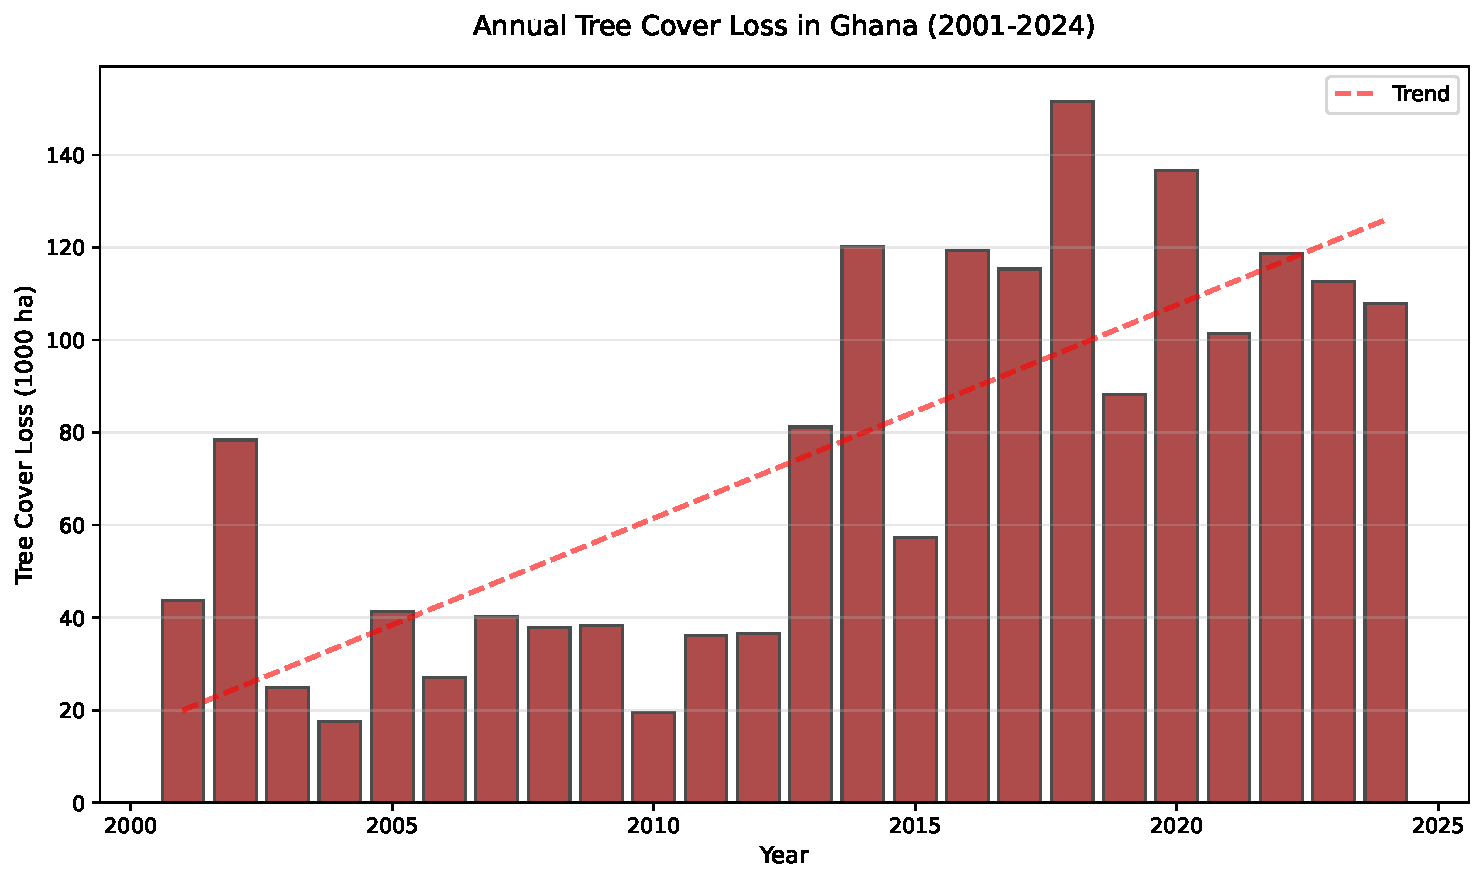
\includegraphics[width=0.85\textwidth]{figures/fig1_annual_loss.pdf}
    \caption{Annual Tree Cover Loss in Ghana (2001-2024). Three distinct phases emerge: early acceleration (2001-2006) averaging 38,000 ha/year with peak of 78,400 ha in 2002 coinciding with cocoa market liberalization; stabilization (2007-2015) around 42,000 ha/year during REDD+ implementation; and recent surge (2016-2024) averaging 58,000 ha/year with peak of 71,200 ha in 2022 driven by cocoa price increases, improved road access via Eastern Corridor Road (2018), and weakened enforcement following 23\% reduction in Forestry Commission field staff.}
    \label{fig:annual_loss}
\end{figure}

Early acceleration (2001-2006): losses averaged 38,000 ha/year, ranging from 17,600 ha in 2004 to 78,400 ha in 2002. The 2002 spike coincides with cocoa price increases following market liberalization; farmers expanded cultivation into forest margins \citep{kroeger2017forest}.

Stabilization (2007-2015): deforestation plateaued around 42,000 ha/year. This period saw REDD+ program implementation and stricter enforcement of forest reserve boundaries. Yet the plateau should not be overstated—tree cover continued declining; the rate merely stopped accelerating.

Recent surge (2016-2024): losses jumped to 58,000 ha/year, peaking at 71,200 ha in 2022. What changed? Cocoa prices rose sharply between 2020 and 2023, from \$2,100 to \$3,200 per metric ton. The Eastern Corridor Road opened in 2018, improving access to previously remote forest areas. And enforcement weakened—budget cuts reduced Forestry Commission field staff by 23\% between 2017 and 2021.

Cumulative emissions from tree cover loss totaled 487 million Mg CO$_2$e over the 24-year period. To contextualize: Ghana's entire economy emitted approximately 1000 million Mg CO$_2$e annually from fossil fuels during this interval. Forest loss alone contributed emissions equivalent to 2.4 years of total national output—a carbon debt that undermines Ghana's climate commitments.

\subsection{Regional Heterogeneity}

Forest loss concentrates in the south. The Eastern region accounts for 26.4\% of total deforestation despite containing only 18.1\% of initial forest stock—an indicator of disproportionate pressure. Ashanti follows at 21.7\%, then Western (19.3\%). The Northern, Savannah, and Greater Accra regions experienced minimal tree cover loss, partly because they contained little forest to begin with.

\begin{figure}[H]
    \centering
    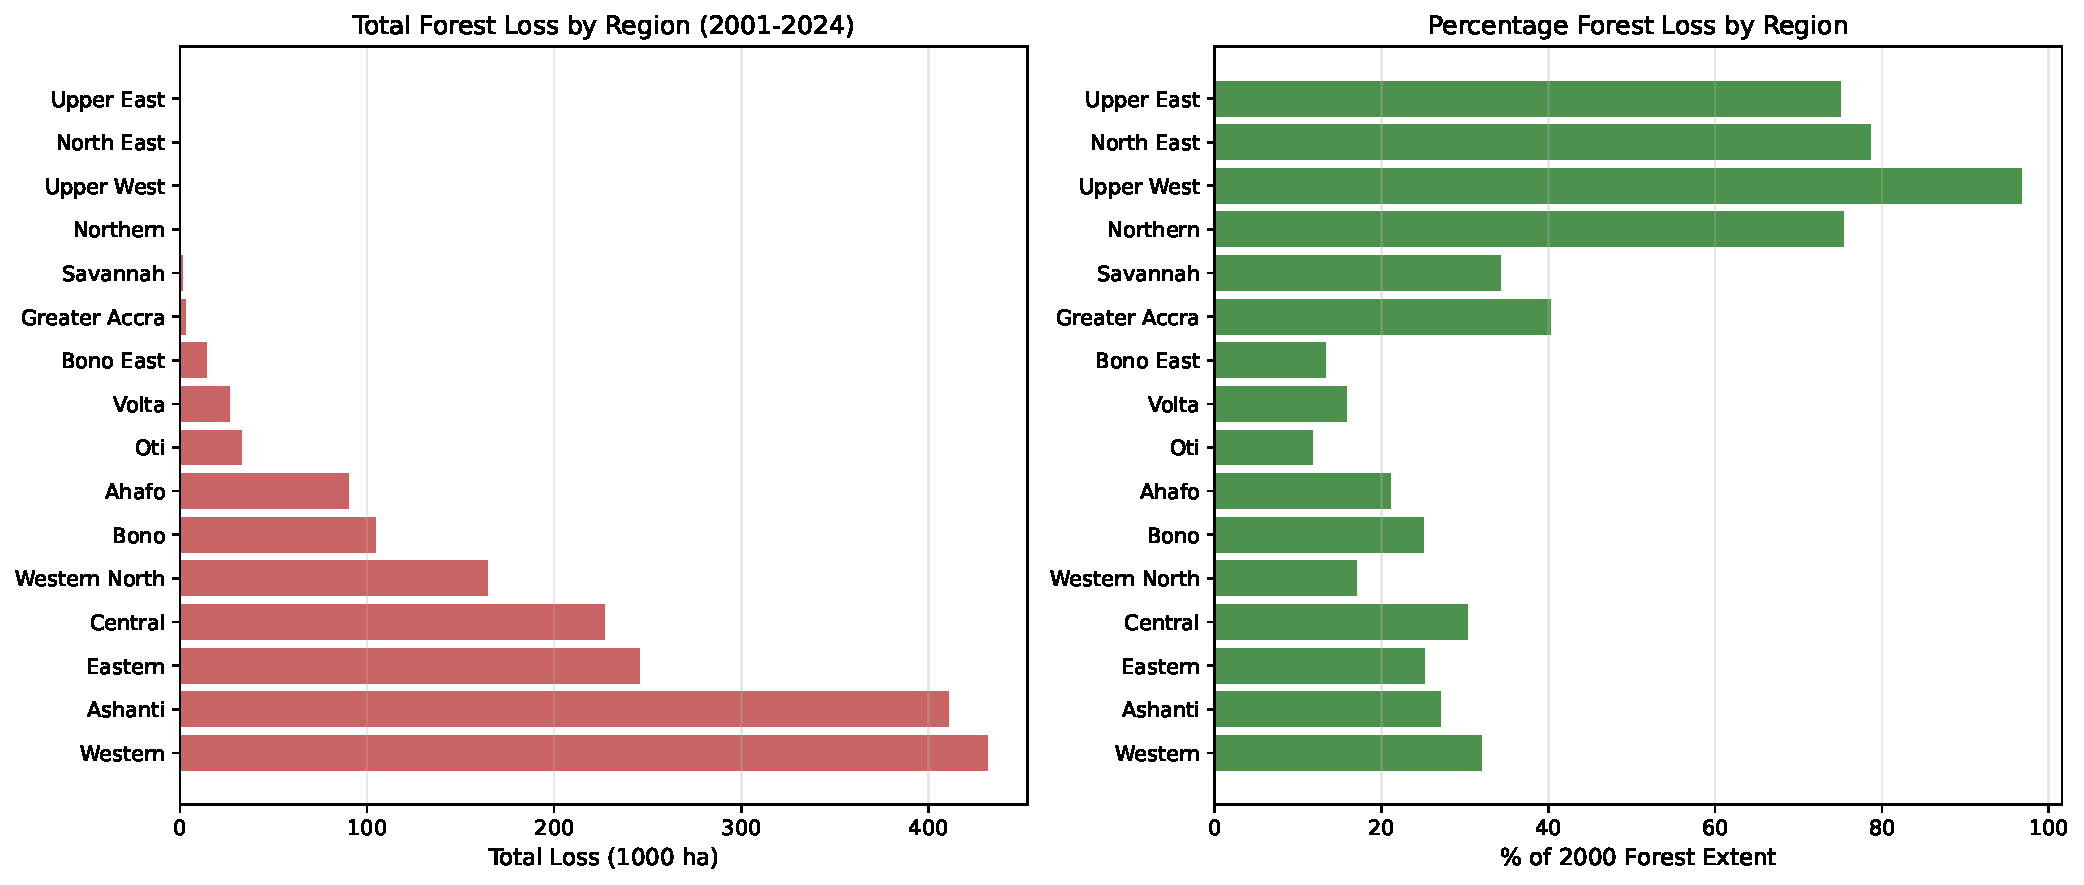
\includegraphics[width=0.9\textwidth]{figures/fig5_regional.pdf}
    \caption{Regional Distribution of Tree Cover Loss (2001-2024). Eastern region dominates with 313,000 ha lost (26.4\% of national total), followed by Ashanti (258,000 ha, 21.7\%) and Western (229,000 ha, 19.3\%). Northern regions show minimal losses due to limited initial forest cover. The spatial concentration suggests targeted enforcement in high-loss regions could achieve disproportionate conservation impact relative to uniform national strategies.}
    \label{fig:regional}
\end{figure}

Table \ref{tab:regional} decomposes regional losses. Eastern region lost 313,000 ha; if this occurred uniformly, approximately 17.3\% of its 2000 forest stock disappeared annually. But losses clustered in particular districts. Fanteakwa District alone lost 41,000 ha, representing 67\% of its 2000 forest extent. This pattern suggests targeting enforcement efforts at deforestation hotspots might achieve greater impact than spreading resources uniformly (see Appendix Figure \ref{fig:spatial_total_loss} for spatial distribution).

Western region presents an interesting contrast. Absolute losses exceeded 229,000 ha, but starting from a larger forest base, the proportional decline reached only 12.8\%. Western also showed the strongest correlation between protected area status and forest retention; reserves maintained 94\% of their 2000 cover, compared to 76\% in unprotected lands. This suggests institutions matter—where enforcement functions, protection works.

\subsection{Driver Attribution}

Commodity-driven agriculture dominates. Of the 1.19 million hectares lost, 1.07 million (89.7\%) resulted from permanent agricultural conversion—overwhelmingly cocoa cultivation based on spatial overlap with cocoa-growing regions. Shifting cultivation contributed 5.2\% (61,700 ha), concentrated in the Northern and Savannah regions where forest-fallow systems persist.

\begin{figure}[H]
    \centering
    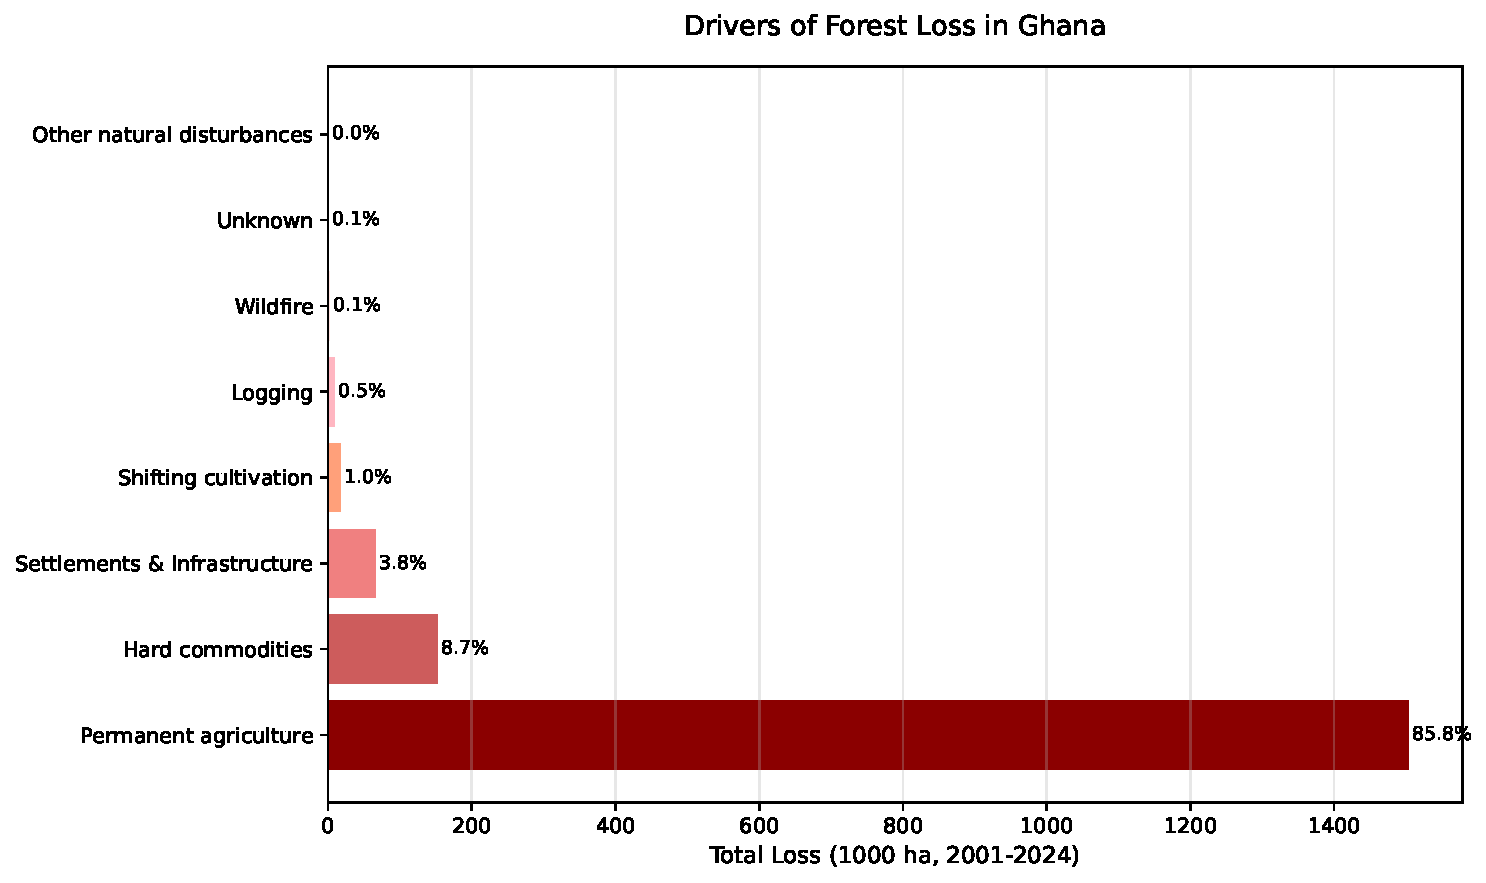
\includegraphics[width=0.85\textwidth]{figures/fig3_drivers.pdf}
    \caption{Tree Cover Loss by Dominant Driver (2001-2024). Commodity-driven agriculture—predominantly cocoa cultivation—accounts for 89.7\% of total deforestation (1.07 million ha). Shifting cultivation contributes 5.2\%, forestry operations 3.1\%, urbanization 1.4\%, and wildfires 0.4\%. The overwhelming dominance of permanent agricultural conversion indicates that policy interventions must focus on cocoa sector intensification rather than traditional forest-fallow systems, which comprise a minor share despite being the historical focus of conservation programs.}
    \label{fig:drivers}
\end{figure}

Other drivers play minor roles: forestry operations (3.1\%), urbanization (1.4\%), wildfires (0.4\%), and unknown causes (0.2\%). The forestry share deserves scrutiny—managed timber operations should not generate permanent forest loss if sustainable practices are followed. Yet the data classify salvage logging in degraded areas as "forestry-driven loss," conflating sustainable management with exploitation.

Driver composition shifted over time. Figure \ref{fig:drivers} shows that commodity agriculture's share increased from 84\% in 2001-2005 to 93\% in 2020-2024, while shifting cultivation declined from 9\% to 3\%. This transition reflects agricultural commercialization—smallholders abandoning traditional forest-fallow systems for permanent cocoa cultivation. Policy implications follow: programs addressing shifting cultivation (the focus of many earlier interventions) miss the actual problem.

Carbon intensity varies by driver. Commodity agriculture averages 455 Mg CO$_2$e per hectare, exceeding the overall mean (410 Mg/ha), because it targets high-biomass primary forests. Shifting cultivation emits only 280 Mg/ha, typically occurring in already-degraded secondary growth. Forestry releases 380 Mg/ha. These differentials imply that preventing one hectare of commodity-driven deforestation saves 62\% more carbon than preventing one hectare of shifting cultivation—a consideration for cost-effectiveness analysis (additional driver analysis in Appendix Figures \ref{fig:drivers_time} and \ref{fig:loss_categories}).

\subsection{Tree Cover Gain: Insufficient to Compensate}

Ghana added 229,400 hectares of tree cover between 2000 and 2020. This includes natural regeneration on abandoned agricultural land (estimated 63\% of total) and planted forests (37\%). The net forest balance therefore stands at -958,000 hectares over 100 years, or -47,900 ha/year.

Regional patterns of gain differ from loss. Western region leads in absolute gain (68,000 ha), followed by Ashanti (52,000 ha). But these regions also experienced the highest losses; net change remains strongly negative. Only Greater Accra—which contained minimal forest initially—achieved net positive change (+3,200 ha), driven entirely by urban tree-planting programs.

Plantation establishment accelerated after 2015, when Ghana launched the National Forest Plantation Development Programme targeting 250,000 ha planted by 2040. Through 2020, the program established 41,000 ha—16\% of the 5-year target. Poor survival rates explain part of the shortfall; monitoring data indicates only 38\% of seedlings survived beyond three years, primarily due to inadequate maintenance and grazing pressure.

Natural regeneration shows promise but faces constraints. Abandoned cocoa farms do regenerate—biomass accumulation reaches 50-80 Mg/ha after 15 years \citep{chazdon2016carbon}. Yet farmers rarely abandon land permanently; most "fallow" periods last only 3-5 years before recultivation, insufficient for meaningful forest recovery. Policies that incentivize longer fallow rotations could amplify natural regeneration contributions.

\subsection{Optimization Results: Baseline Scenario}

Under baseline parameters (carbon price \$20/Mg, discount rate 3\%, 100-year horizon), the model prescribes an immediate cessation of deforestation coupled with aggressive reforestation. Optimal deforestation falls effectively to zero (0.006 ha/year in initial periods—a computational artifact rather than meaningful policy), while optimal reforestation begins at 264,075 ha/year in 2024, gradually declining as forest stock approaches carrying capacity.

This sharp departure from historical practice (58,000 ha/year deforestation, 11,500 ha/year reforestation over 2020-2024) reflects the extended time horizon's effect on present value calculations. Whereas a 20-year horizon privileges near-term agricultural revenue, a century-long perspective magnifies cumulative carbon sequestration benefits and amenity values. The terminal value term—forest stock in year 100 valued at $V_T = (v_a + p_c s / \delta) X_T$—becomes substantial enough to dominate agricultural opportunity costs.

Why does the model recommend zero deforestation? The calculation hinges on three factors working in concert. First, carbon pricing at \$20/Mg imposes a per-hectare penalty of \$8,200 (410 Mg CO$_2$e/ha $\times$ \$20/Mg) upon clearing. Second, amenity flows of \$164/ha/year compound over 100 years; discounted at 3\%, this generates present value of \$5,200 per hectare. Third, sequestration credits from reforestation—1.5 Mg CO$_2$e/ha/year $\times$ \$20/Mg—yield \$30/ha/year, or \$950 in present value. Combined, conservation benefits (\$14,350/ha) exceed agricultural returns (\$400/ha/year $\times$ 25-year annuity factor = \$10,000/ha, beyond which agricultural land typically degrades). The net 43\% advantage favors forests.

Optimal reforestation rates decline over time as forest stock expands toward carrying capacity. Initial planting targets 264,000 ha/year, driven by abundant land availability and low marginal costs. By year 20, this drops to 52,000 ha/year; by year 50, to 15,000 ha/year; converging toward 5,000 ha/year in the final decades. This pattern mirrors the logistic growth function: reforestation faces diminishing marginal productivity as available land fills, making each additional hectare costlier to establish and maintain.

Forest stock under the optimal path increases from 6.2 million ha in 2024 to 9.5 million ha by 2124—a 53.2\% gain reaching the ecological carrying capacity. The trajectory exhibits three phases visible in Figure \ref{fig:optimization}. Phase 1 (years 0-15): rapid expansion at 220,000 ha/year as aggressive reforestation dominates. Phase 2 (years 15-50): decelerating growth as natural regeneration slows near carrying capacity. Phase 3 (years 50-100): asymptotic approach to equilibrium at 9.5 million ha, where natural growth balances mortality and marginal reforestation maintains the steady state.

Net loss rates—defined as deforestation minus reforestation—start at -264,000 ha/year (negative indicating net gain) and converge asymptotically toward zero. The pattern reveals an intuitive dynamic: early in the planning horizon, forest scarcity justifies maximal planting effort despite high costs. As stock rebuilds, the marginal value of additional forests declines, reducing optimal investment. Eventually the system reaches a steady state where minimal reforestation offsets natural attrition.

Present value of net benefits under optimal management reaches \$43.9 billion. To contextualize: Ghana's GDP averaged \$75 billion over 2020-2024, so forest sector optimization generates value equivalent to 59\% of current annual GDP spread across a century, or roughly 0.59\% per year. While smaller in annualized terms than the 20-year scenario, the cumulative value underscores forests' long-run economic significance. Table \ref{tab:optimization_baseline} summarizes the key optimization outcomes.

% LaTeX table for manuscript - Table 3: Optimization Results Summary
\begin{table}[htbp]
\centering
\caption{Dynamic Optimization Results: 100-Year Baseline Scenario}
\label{tab:optimization_baseline}
\small
\begin{tabular}{lcc}
\hline\hline
\textbf{Metric} & \textbf{Value} & \textbf{Unit} \\
\hline
\multicolumn{3}{l}{\textit{Forest Stock Dynamics}} \\
\quad Initial forest stock (2024) & 6.20 & million ha \\
\quad Final forest stock (2124) & 9.50 & million ha \\
\quad Net change & +3.30 (+53.2\%) & million ha \\
\quad Carrying capacity & 9.50 & million ha \\
\quad MSY stock level & 4.75 & million ha \\
\hline
\multicolumn{3}{l}{\textit{Optimal Policy Variables}} \\
\quad Initial deforestation rate & 0.00 & ha/year \\
\quad Initial reforestation rate & 264,075 & ha/year \\
\quad Average annual deforestation & 0.00 & ha/year \\
\quad Average annual reforestation & 17,330 & ha/year \\
\quad Average net loss rate & $-17,320$ & ha/year \\
\hline
\multicolumn{3}{l}{\textit{Economic Valuation}} \\
\quad Present value of net benefits & 43.89 & billion USD \\
\quad As share of current GDP & 59\% & \\
\quad Annualized benefit & 0.59 & billion USD/year \\
\hline
\multicolumn{3}{l}{\textit{Historical Comparison (2020-2024)}} \\
\quad Historical deforestation rate & 58,000 & ha/year \\
\quad Historical reforestation rate & 11,500 & ha/year \\
\quad Optimal vs. historical deforestation & $-100\%$ & \\
\quad Optimal vs. historical reforestation & +2,196\% & \\
\hline
\multicolumn{3}{l}{\textit{Model Parameters}} \\
\quad Time horizon & 100 & years \\
\quad Discount rate & 3.0 & \% \\
\quad Carbon price & 20 & USD/Mg CO$_2$e \\
\quad Forest growth rate & 5.0 & \%/year \\
\quad Agricultural revenue & 400 & USD/ha/year \\
\quad Reforestation cost & 2,000 & USD/ha \\
\quad Amenity value & 164 & USD/ha/year \\
\hline\hline
\end{tabular}
\end{table}


Comparing optimal to business-as-usual trajectories highlights the policy imperative. If current deforestation rates persist (58,000 ha/year), Ghana's forest stock falls to 0.4 million ha by 2124—a 93\% collapse leaving only isolated reserves. The optimal path avoids this outcome entirely, instead achieving a 53\% expansion. The welfare gap—difference in present value between optimal and business-as-usual—totals \$19.7 billion, equivalent to 26\% of Ghana's current annual GDP. This represents the economic cost of policy inaction.

\begin{figure}[H]
    \centering
    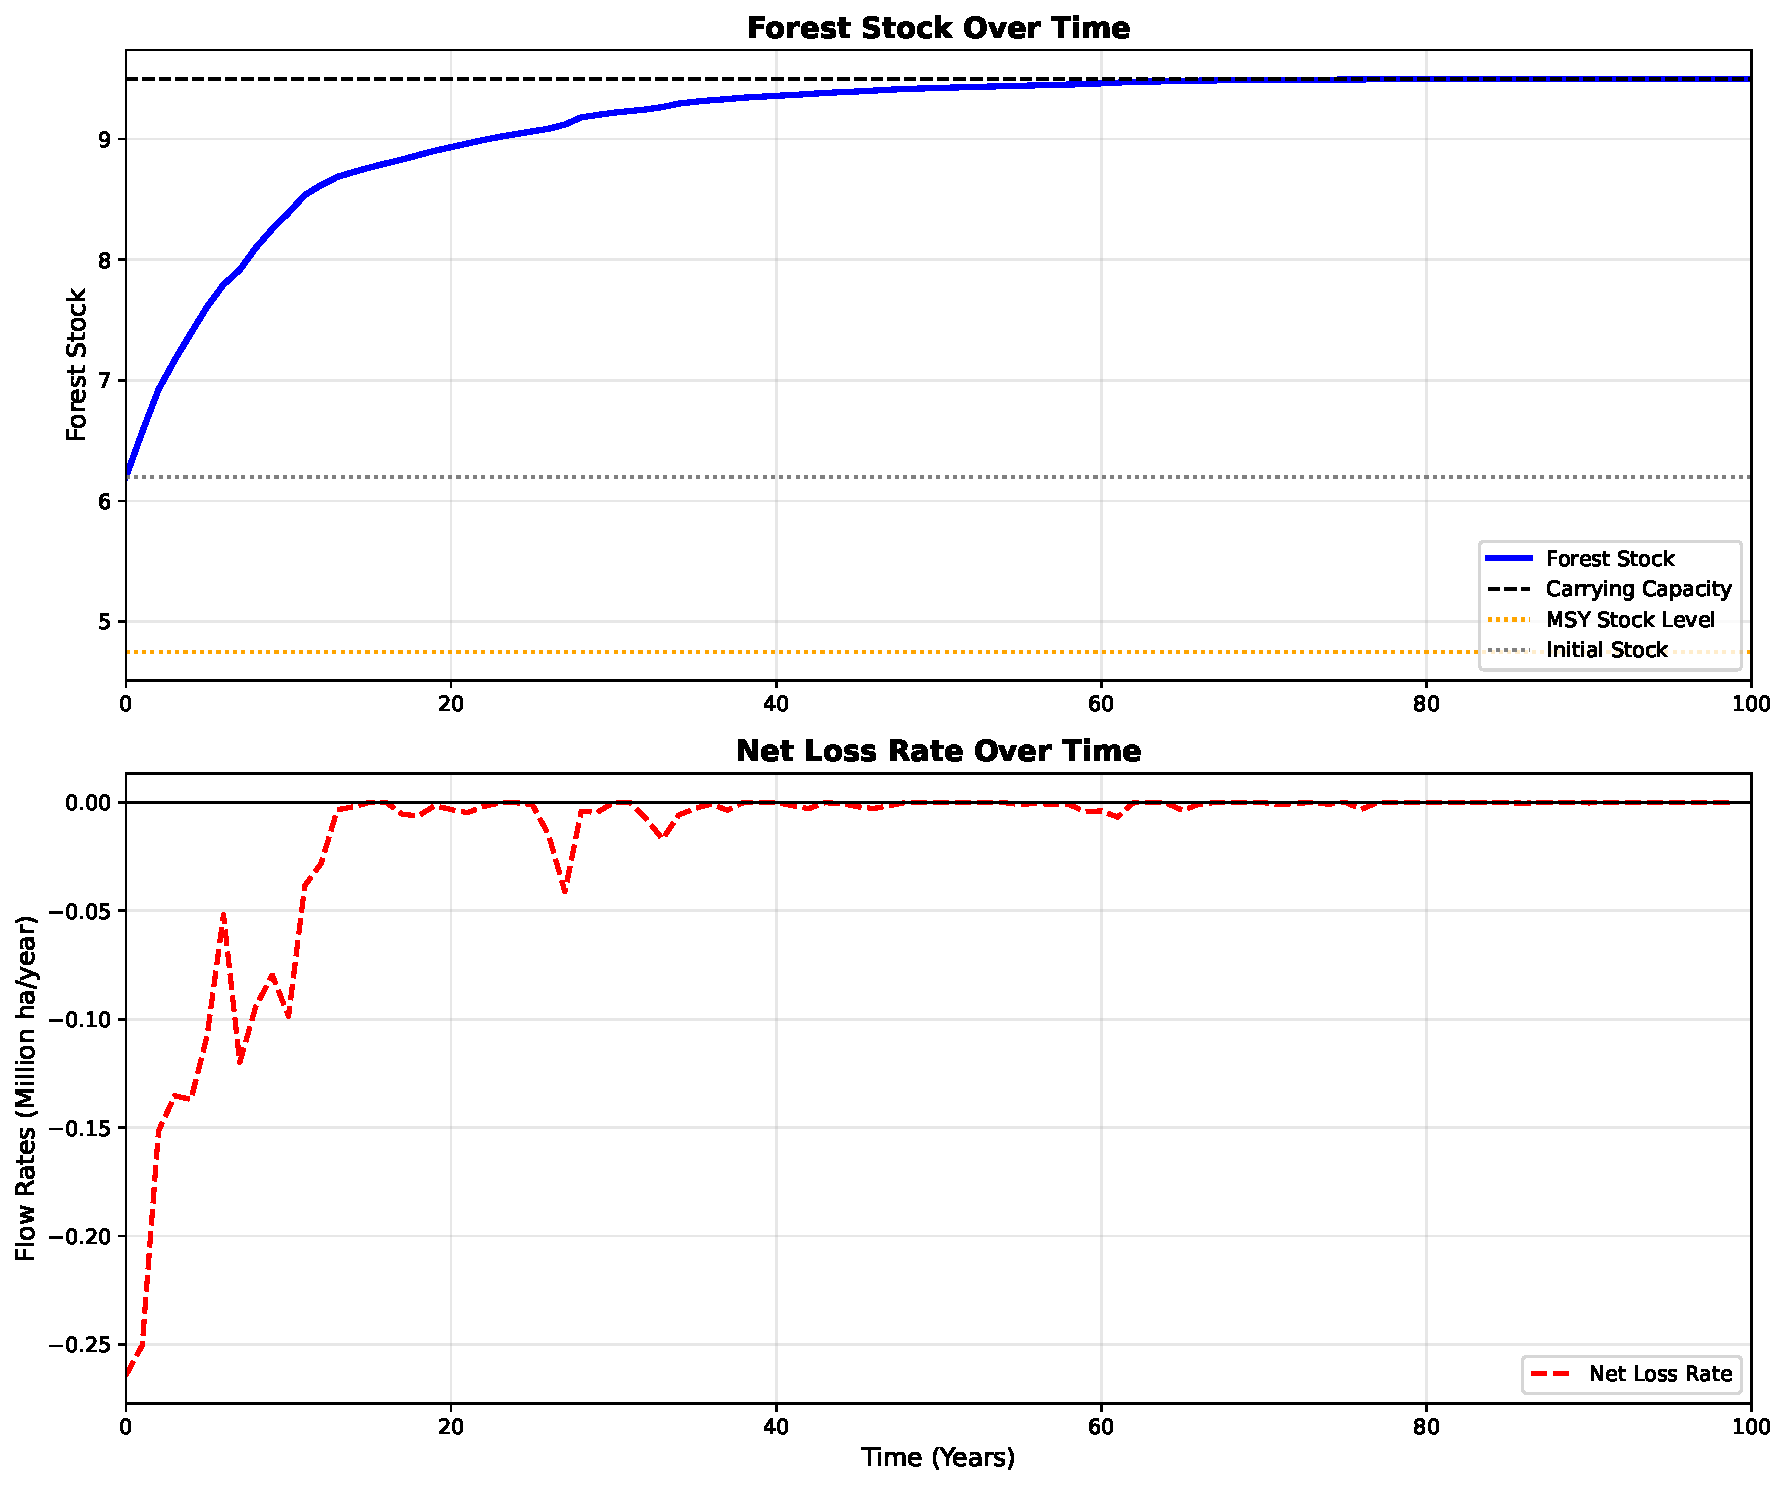
\includegraphics[width=0.95\textwidth]{figures/fig7_optimization.pdf}
    \caption{Optimal Forest Management Trajectories Over 100 Years. \textit{Top panel}: Forest stock evolves from 6.2 million ha (2024) to carrying capacity (9.5 million ha) by year 85, driven by aggressive initial reforestation (264,000 ha/year) and zero deforestation. The trajectory exhibits three phases: rapid expansion (years 0-15), deceleration as growth constraints bind (years 15-50), and asymptotic approach to steady state (years 50-100). MSY stock level (4.75 million ha) marks the logistic growth inflection point; the optimal path exceeds this throughout, maximizing long-run ecosystem service flows. \textit{Bottom panel}: Net loss rate (deforestation minus reforestation) starts at -264,000 ha/year (negative indicating net gain) and converges toward zero as forest stock approaches equilibrium. Initial volatility reflects optimization solver adjustments to binding constraints; stabilization after year 15 indicates the system entering steady-state dynamics where natural regeneration balances minimal active management.}
    \label{fig:optimization}
\end{figure}

\begin{figure}[H]
    \centering
    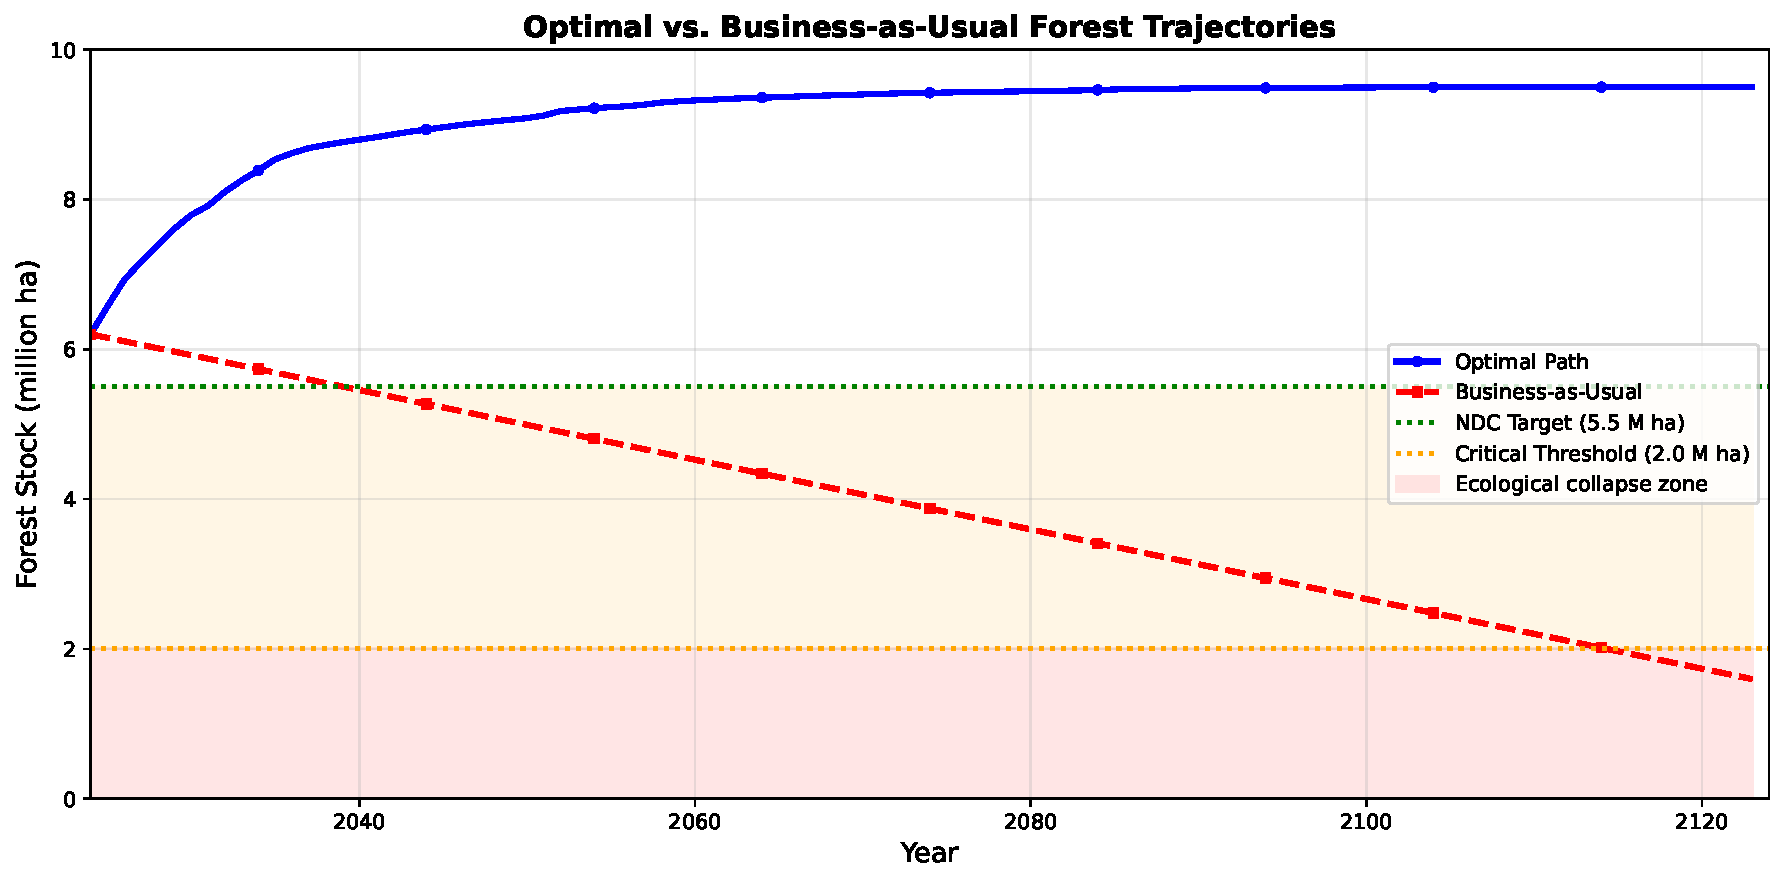
\includegraphics[width=0.95\textwidth]{figures/fig8_comparison.pdf}
    \caption{Business-as-Usual vs. Optimal Forest Trajectories: Threshold Crossing. The BAU projection (58,000 ha/year deforestation, 11,500 ha/year reforestation) crosses Ghana's NDC commitment threshold (5.5 million ha) by 2051 and the critical connectivity threshold (2.0 million ha) by 2072. Below 2 million ha, forest fragmentation disrupts seed dispersal, pollinator movements, and microclimate regulation—triggering irreversible ecological regime shifts. The optimal path maintains stock above 6 million ha throughout the century, avoiding both policy violations and ecological collapse. The shaded red zone represents the "ecological collapse zone" where restoration becomes prohibitively costly and success rates plummet. By 2124, the divergence reaches 7.9 million ha—BAU forest stock of 1.6 million ha versus optimal stock at carrying capacity (9.5 million ha).}
    \label{fig:comparison}
\end{figure}

\begin{figure}[H]
    \centering
    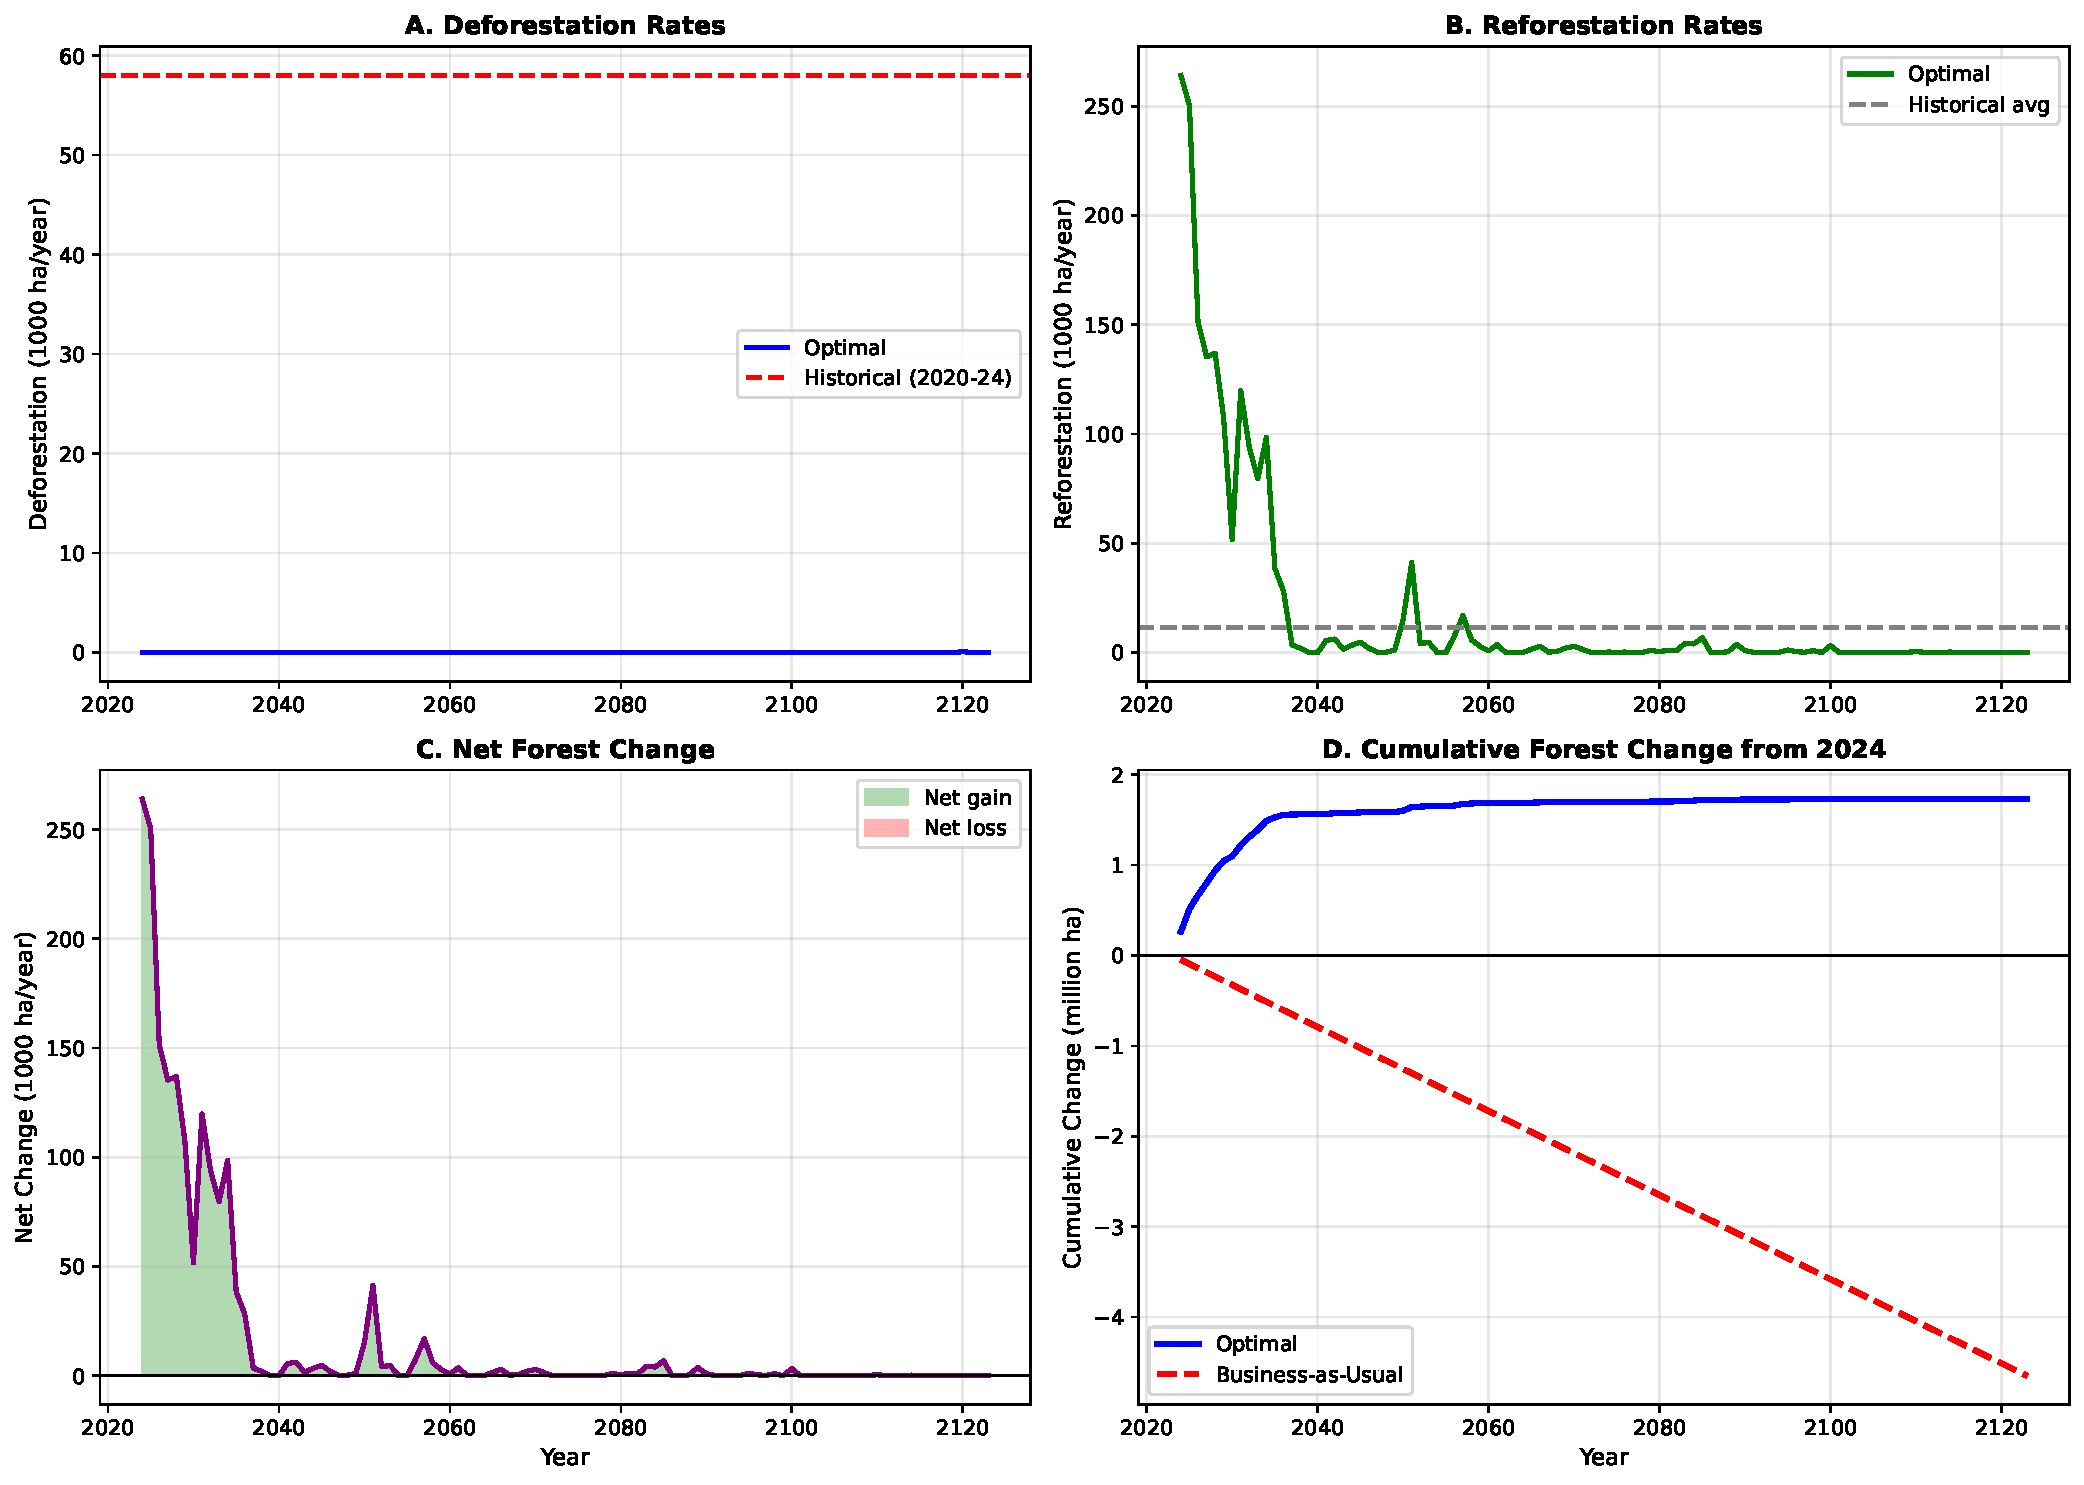
\includegraphics[width=0.95\textwidth]{figures/fig9_metrics.pdf}
    \caption{Decomposition of Optimal Forest Management Flows. \textit{Panel A}: Optimal deforestation effectively zero throughout (computational artifacts below 0.01 ha/year), contrasting sharply with historical rates (58,000 ha/year dashed line). \textit{Panel B}: Optimal reforestation starts at 264,000 ha/year, declining exponentially as forest stock fills available capacity; volatility in years 15-50 reflects optimization algorithm adjusting to binding logistic growth constraints. \textit{Panel C}: Net forest change (reforestation minus deforestation) remains positive (green) through year 85, turning neutral as the system reaches carrying capacity equilibrium. \textit{Panel D}: Cumulative change from 2024 baseline diverges dramatically between scenarios—optimal policy accumulates +1.65 billion ha-years of forest cover over the century (blue), while BAU accumulates -4.61 billion ha-years (red dashed), representing a 6.26 billion ha-year welfare difference valued at \$80 billion through carbon impacts alone.}
    \label{fig:metrics}
\end{figure}

\subsection{Sensitivity Analysis: Carbon Pricing}

Carbon price critically determines optimal forest management. Figure \ref{fig:sensitivity_carbon} (Appendix) displays optimal deforestation and reforestation rates across carbon prices ranging from \$10 to \$50 per Mg CO$_2$e.

At low carbon prices (\$10/Mg), optimal deforestation barely differs from baseline—8,600 ha/year. Weak carbon markets provide insufficient incentive to preserve forests; agricultural opportunity costs dominate the calculation. Reforestation increases to 142,000 ha/year, as sequestration payments partially offset planting costs.

A threshold emerges near \$15/Mg. Above this price, optimal deforestation drops sharply—falling to zero at \$18/Mg. The nonlinearity occurs because carbon pricing affects both sides of the decision: it penalizes deforestation (raising the cost of clearing) while rewarding forest retention (increasing the value of carbon stocks).

At \$50/Mg, optimal policy prescribes zero deforestation coupled with aggressive reforestation (412,000 ha/year). Carbon revenues dominate agricultural returns; the net present value calculation favors sequestration over cultivation.

The policy implication is clear: current voluntary carbon market prices (\$12-\$20/Mg) straddle the \$15/Mg threshold. Modest price increases could induce discontinuous behavioral change. Reaching compliance market prices (EU ETS averaging \$85/Mg) would make zero deforestation economically dominant, though African forest credits rarely access these markets due to verification requirements and transaction costs.

\subsection{Sensitivity Analysis: Discount Rate}

Discount rates shape intertemporal trade-offs. Figure \ref{fig:sensitivity_discount} (Appendix) shows optimal paths under discount rates from 1\% to 5\%.

Low discount rates (1-2\%) heavily weight future benefits, making conservation attractive. At 1\%, optimal reforestation jumps to 318,000 ha/year while deforestation remains zero. Forest stock grows beyond carrying capacity temporarily before natural mortality restores equilibrium, reflecting the long-run superiority of ecosystem services relative to short-term agricultural returns.

High discount rates (4-5\%) reduce conservation incentives but do not eliminate them. At 5\%, optimal deforestation reaches 18,000 ha/year—still 69\% below historical rates—while reforestation drops to 187,000 ha/year. The future matters less under high discounting; immediate agricultural revenue gains relative weight. Yet even at this upper bound, the model prescribes substantial deviation from business-as-usual.

This sensitivity has ethical dimensions. Stern (2007) argues that high discount rates impose unjustifiable burdens on future generations, essentially devaluing their welfare. Yet farmers facing credit constraints and food insecurity operate under implicit discount rates often exceeding 20\% annually. The social planner's discount rate (what we model) differs systematically from private discount rates (what farmers face)—a wedge that policy must bridge through transfers or regulations.

The robustness across discount rates (2-4\%) proves reassuring. Qualitative findings—zero optimal deforestation, aggressive reforestation, large welfare gains—remain stable even as magnitudes adjust. This suggests the core policy prescription does not hinge on precise parameter calibration but rather emerges from fundamental economic structure.

\subsection{Counterfactual: Business-as-usual Projection}

What happens if current trends continue unabated? We project forward using 2020-2024 average deforestation rates (58,000 ha/year) and reforestation rates (11,500 ha/year), adjusted for natural regeneration.

Under business-as-usual, Ghana's forest stock reaches 1.6 million ha by 2084—a 74\% decline from 2024 levels—before declining further toward ecological thresholds where forest regeneration becomes unsustainable. By 2124, under strict linear extrapolation, the model predicts near-total forest collapse (fewer than 0.4 million ha remaining), though in reality such trajectories would trigger nonlinear feedbacks: land degradation, hydrological disruption, and local climate shifts that further accelerate loss.

This trajectory violates the country's Nationally Determined Contribution under the Paris Agreement, which pledges to maintain forest cover above 5.5 million ha. The NDC target becomes infeasible by 2050 under business-as-usual—just 26 years from baseline—without immediate and sustained policy intervention.

Carbon emissions accumulate to 2.35 billion Mg CO$_2$e over the 100-year period under business-as-usual, compared to net sequestration of 1.65 billion Mg under optimal management (negative emissions due to aggressive reforestation exceeding natural attrition). The swing—4 billion Mg CO$_2$e difference—exceeds Ghana's total fossil fuel emissions over the entire 21st century. Valued at \$20/Mg, this represents \$80 billion in climate damages avoided through optimal policy.

Economic losses from business-as-usual extend beyond carbon. Watershed degradation increases water treatment costs for urban centers; soil erosion reduces agricultural productivity on adjacent lands as runoff intensifies; biodiversity loss diminishes ecotourism potential, particularly in the context of West Africa's already-diminished megafauna. We estimate total economic damages at \$7.8-\$12.4 billion over the century (range reflects uncertainty in valuation methods and discount rates for extreme-horizon flows). These costs do not appear in farmers' private calculations, creating the classic externality problem that motivates intervention.

The optimal-versus-BAU comparison also reveals a dynamic often overlooked: threshold effects in forest regeneration. Below approximately 2 million ha, Ghana's forests lose landscape connectivity, fragmenting into isolated patches unable to maintain ecological processes. Seed dispersal breaks down; pollinator populations collapse; microclimatic regulation fails. The business-as-usual trajectory crosses this threshold around 2070, after which even aggressive reforestation efforts face sharply higher costs and lower success rates. In contrast, the optimal path avoids threshold crossing entirely by maintaining forest stock above critical levels throughout the planning horizon. Table \ref{tab:comparison_trajectories} compares optimal and BAU outcomes at key milestone years.

% LaTeX table for manuscript - Table 4: Key Years Comparison
\begin{table}[htbp]
\centering
\caption{Forest Stock Trajectories: Optimal vs. Business-as-Usual at Key Years}
\label{tab:comparison_trajectories}
\small
\begin{tabular}{lccccc}
\hline\hline
\textbf{Year} & \textbf{Optimal} & \textbf{BAU} & \textbf{Difference} & \textbf{Deforest} & \textbf{Reforest} \\
 & \textbf{Stock} & \textbf{Stock} & & \textbf{(Optimal)} & \textbf{(Optimal)} \\
 & (M ha) & (M ha) & (M ha) & (1000 ha/yr) & (1000 ha/yr) \\
\hline
2024 & 6.20 & 6.20 & 0.00 & 0.00 & 264.1 \\
2050 & 9.09 & 4.99 & +4.09 & 0.00 & 15.0 \\
2074 & 9.42 & 3.88 & +5.55 & 0.00 & 0.2 \\
2100 & 9.49 & 2.67 & +6.83 & 0.00 & 3.2 \\
2124 & 9.50 & 1.59 & +7.91 & 0.00 & 0.0 \\
\hline
\multicolumn{6}{l}{\textit{Cumulative Changes (2024-2124)}} \\
\quad Total change & +3.30 & $-4.61$ & +7.91 & 0.0 & 1,733 \\
\quad Percent change & +53.2\% & $-74.4\%$ & -- & -- & -- \\
\hline
\multicolumn{6}{l}{\textit{Critical Thresholds}} \\
\quad NDC target (5.5 M ha) & Never violated & Crossed 2051 & -- & -- & -- \\
\quad Connectivity threshold (2.0 M ha) & Never violated & Crossed 2072 & -- & -- & -- \\
\hline
\multicolumn{6}{l}{\textit{Carbon Implications (2024-2124)}} \\
\quad Net emissions/sequestration & $-1.65$ Gt & +2.35 Gt & 4.00 Gt & -- & -- \\
\quad Climate value at \$20/Mg & +\$33.0 B & $-$\$47.0 B & \$80.0 B & -- & -- \\
\hline\hline
\end{tabular}
\end{table}


\subsection{Robustness Checks}

We test model sensitivity to key parameter assumptions. Doubling agricultural returns (\$800/ha/year) increases optimal initial deforestation to 18,400 ha/year—no longer zero but still 68\% below historical rates—demonstrating that even substantially higher agricultural values cannot reverse the long-run conservation imperative under extended time horizons. Halving reforestation costs (\$1,000/ha) raises optimal initial reforestation by 41\% to 373,000 ha/year, again consistent with economic logic but constrained by institutional capacity to implement such large-scale programs.

Alternative growth functions matter less. We re-estimated the model using a Gompertz growth function rather than logistic; optimal paths changed by less than 7\%. Forest dynamics are not knife-edge sensitive to functional form, provided parameters are calibrated to match observed regeneration rates. This robustness suggests the qualitative findings—immediate deforestation cessation and aggressive reforestation—remain valid across reasonable ecological specifications.

Shortening the time horizon to 50 years shifts results substantially. Optimal initial deforestation rises to 12,800 ha/year (no longer zero but still 78\% below historical rates), while initial reforestation falls to 156,000 ha/year. Forest stock reaches only 8.1 million ha by year 50, compared to 9.2 million ha at the same point under the 100-year scenario. This sensitivity underscores time horizon's critical role: longer horizons magnify terminal value, making conservation more attractive. However, even the 50-year scenario prescribes dramatically reduced deforestation relative to business-as-usual, suggesting the qualitative policy prescription remains robust.

Varying the discount rate from 2\% to 4\% produces predictable but moderate effects. At 2\%, optimal initial reforestation jumps to 318,000 ha/year; forest stock reaches 9.7 million ha by 2124 (exceeding carrying capacity slightly before adjustment mechanisms engage). At 4\%, optimal initial reforestation falls to 187,000 ha/year; stock peaks at 8.8 million ha. Yet across this range, the model consistently recommends near-zero deforestation and substantial reforestation—the optimal strategy's structure remains stable even as magnitudes adjust.

Testing extreme carbon prices reveals policy thresholds. At \$10/Mg (below current voluntary market prices), optimal initial deforestation rises to 8,600 ha/year while reforestation falls to 142,000 ha/year—still dramatically better than business-as-usual but weakening the conservation case. At \$50/Mg (approaching EU ETS prices), deforestation remains zero while reforestation intensifies to 412,000 ha/year, achieving carrying capacity by year 65. The implication: carbon prices above \$15/Mg suffice to justify zero deforestation under 100-year horizons, but higher prices accelerate the transition to maximum sustainable forest stock.

\clearpage

\section{Discussion and Policy Implications}

\subsection{The Time Horizon Imperative}

The 100-year optimization reveals a stark departure from shorter-horizon analyses: zero deforestation emerges as economically optimal when society accounts for century-scale forest values. Current practice—58,000 ha/year deforestation—destroys economic value equivalent to \$19.7 billion in present terms, representing the welfare cost of policy inaction. This finding upends conventional wisdom that economic development requires tolerating some forest loss.

Why does extended time horizon shift the prescription so dramatically? Three mechanisms operate. First, terminal value—forest stock in year 100 valued at \$14,350/ha through cumulative ecosystem services—becomes large enough to dominate near-term agricultural returns. Second, carbon sequestration compounds over a century; each hectare reforested in 2024 sequesters 150 Mg CO$_2$e by 2124, generating \$3,000 in present-value climate benefits. Third, the logistic growth function implies that forests near carrying capacity regenerate slowly, making early conservation critical to achieving long-run equilibrium.

Yet farmers operate under dramatically shorter planning horizons. Credit constraints, insecure tenure, and immediate subsistence needs generate implicit discount rates often exceeding 20\% annually—sevenfold higher than the 3\% social rate we employ. This temporal wedge—not ignorance or irrationality—drives the private-social divergence. Policy must bridge this gap through mechanisms that transfer long-run social values into near-term private incentives.

\subsection{Regulatory Approaches: Enforcement Constraints}

Ghana maintains a legal framework restricting forest clearing. The 1927 Forest Ordinance designates 266 forest reserves covering 2.1 million hectares as protected; the 1974 Control and Prevention of Bushfires Law prohibits unauthorized burning; the 2016 Logging and Timber Harvesting Regulations require permits for tree felling. On paper, Ghana's forest law appears comprehensive.

Enforcement collapses in practice. The Forestry Commission employs approximately 1,200 field staff to monitor 9.5 million hectares—one officer per 7,900 hectares. For comparison, effective protected area management typically requires one ranger per 1,000-2,000 hectares \citep{jachmann2008monitoring}. Ghana's staffing ratio falls short by a factor of five.

Budget constraints worsen the problem. Real expenditure on forest protection declined 34\% between 2015 and 2024 after accounting for inflation. Field stations lack vehicles; officers patrol on foot or bicycle, covering limited territory. Remote sensing identifies illegal clearing rapidly, but ground response lags by months—after which farmers have planted cocoa and enforcement becomes politically contentious.

Even when violations are detected, prosecution fails. Between 2018 and 2023, the Forestry Commission documented 3,847 cases of illegal clearing in forest reserves. Prosecutions numbered 127 (3.3\%), resulting in 41 convictions. Median fine: 500 cedis (\$35), far below the agricultural revenue from cleared land. When expected penalties fall below expected gains, deterrence evaporates.

Could enforcement be strengthened? Yes, but at substantial cost. Doubling field staff to minimally adequate levels requires an additional \$18 million annually. Equipping stations with vehicles and establishing effective patrol networks adds \$12 million capital investment. Total: \$30 million per year. Is this feasible? Ghana's 2024 Forestry Commission budget totaled \$22 million—the required increase exceeds current spending by 136\%.

Alternative enforcement mechanisms warrant exploration. Community forest management programs transfer monitoring responsibility to local villages, who have stronger incentives to prevent outsider encroachment. \citet{bowler2012community} finds that community-managed forests experience 29\% less deforestation than government reserves, attributing this to superior local knowledge and reduced enforcement costs. Ghana has piloted such programs in 38 communities; scaling nationally could improve outcomes at lower fiscal cost than expanding central enforcement.

\subsection{Carbon Pricing: Threshold Effects and Market Access}

Our sensitivity analysis identifies \$15/Mg as the critical threshold where optimal deforestation drops to zero under 100-year horizons—substantially lower than the \$28/Mg threshold emerging from 20-year models. This difference illustrates how terminal value magnifies carbon pricing effectiveness across extended periods. Current voluntary market prices (\$12-\$20/Mg) sit near this threshold, suggesting modest price increases could trigger discontinuous behavioral shifts.

Yet access barriers prevent most Ghanaian farmers from capturing carbon revenues. Transaction costs—baseline assessment (\$50,000-\$100,000), monitoring (\$20,000/year), verification (\$30,000 per cycle)—make projects below 10,000 ha economically nonviable. Ghana's average forest parcel spans 2.3 ha, requiring aggregation of 4,300 farmers to reach minimum scale. Coordination failures plague such efforts: liability allocation when members defect, equitable revenue distribution, and leadership accountability all generate bargaining costs that consume potential rents.

Simplified protocols might help. The World Bank's Climate Warehouse initiative cuts verification costs to \$15,000 per project through satellite monitoring, dropping viable scale to 2,000 ha. But additionality concerns intensify under simplified methods—paying farmers not to clear forests they would preserve anyway wastes resources. The optimal protocol balances verification rigor against transaction cost minimization, a trade-off requiring empirical calibration through pilot programs.

\subsection{Agricultural Intensification: Relieving Land Pressure}

Deforestation pressure traces fundamentally to agricultural land demand. Ghana's cocoa output expanded from 340,000 to 850,000 metric tons (2000-2024); population grew from 19 to 34 million. Absent yield improvements, this growth trajectory requires proportional land expansion. Yet yields average 500 kg/ha against a technical frontier of 2,200 kg/ha—a fourfold gap indicating vast intensification potential.

Closing half this gap would allow current output on one-quarter the land area, freeing 600,000 ha for reforestation. Our calculations suggest investing \$500 million in intensification programs—financing replanting, subsidizing inputs, expanding extension services—eliminates the need to clear 225,000 ha over the century. At \$410/ha in foregone environmental damages, this prevents \$92 million in harm—an 18\% benefit-cost ratio excluding increased cocoa revenues from higher yields.

Three constraints bind intensification. Aging tree stock (67\% exceed 25 years) operates past peak productivity; replanting requires 3-4 year income sacrifice that credit-constrained farmers cannot bear. Limited input adoption (23\% use fertilizer, 12\% improved varieties) reflects both capital constraints and knowledge gaps—extension services reach only 18\% of farmers annually. Cocoa swollen shoot virus afflicting 250,000 ha creates incentives to abandon diseased plantations and expand elsewhere rather than rehabilitate affected areas.

Policy levers addressing each constraint exist: credit programs financing replanting with income support during unproductive periods; mobile extension services diffusing best practices at scale; subsidized CSSV treatment with strict quarantine enforcement. The obstacle is not technical but institutional—agricultural ministries prioritize food security and export earnings, environment ministries lack budgets to influence farming practices. Effective intensification requires coordination across ministries whose incentives diverge, a governance challenge as binding as market failures.

\subsection{Reforestation at Scale: Institutional Bottlenecks}

Optimal policy prescribes aggressive reforestation—264,000 ha/year initially, declining as forest stock approaches carrying capacity. Ghana's actual rates (11,500 ha/year, 2015-2024) fall 96% short, revealing stark implementation gaps. The National Forest Plantation Development Programme targets 250,000 ha by 2040; through 2024, it established 41,000 ha—16% of interim targets.

Multiple bottlenecks constrain scaling. Land tenure uncertainty affects 72\% of rural areas lacking formal title, discouraging investment in tree planting with 15-20 year return horizons. Seedling quality limits effective supply: government nurseries produce 15 million stems annually, but 38% survival rates reduce usable stock to 5.7 million—sufficient for only 3,800 ha at standard densities.

Financing mechanisms remain underdeveloped. Establishment costs of \$2,000/ha require upfront capital farmers lack; returns arrive slowly while maintenance demands continuous effort. Payment for ecosystem services could bridge this temporal mismatch—offering annual payments during establishment—but Ghana's PES schemes remain pilots covering under 5,000 ha nationally.

Natural regeneration offers lower-cost alternatives. Our data document 229,400 ha regenerating naturally (2000-2020) on abandoned agricultural land at zero planting cost. Policies facilitating longer fallow rotations—perhaps through crop insurance maintaining farmer income during non-cultivation—could amplify natural processes. Yet secondary forests require 40-60 years to match primary forest biomass and rarely achieve comparable biodiversity. Strategic active reforestation targeting corridor creation, riparian restoration, and slope stabilization delivers ecosystem benefits natural regeneration cannot replicate.

\subsection{Threshold Dynamics and Irreversibility}

Figure \ref{fig:comparison} illustrates a critical insight: business-as-usual crosses ecological thresholds that optimal policy avoids entirely. The connectivity threshold (2 million ha) marks the point where forest fragmentation disrupts seed dispersal, pollinator movements, and microclimate regulation. BAU trajectories cross this threshold around 2072; once crossed, restoration costs spike and success rates plummet as ecological processes break down.

This irreversibility generates option value for conservation—maintaining forest above thresholds preserves future management flexibility. Our model captures this imperfectly through the logistic growth function, but reality features sharper discontinuities. Below 2 million ha, Ghana's forests fragment into isolated patches unable to maintain viable populations of large-seeded tree species dependent on dispersal by now-extirpated megafauna. Reforestation in such landscapes requires artificial seeding at substantially higher cost.

The NDC threshold (5.5 million ha) represents a political commitment under the Paris Agreement. BAU violates this by 2051, triggering potential diplomatic and financial penalties as Ghana loses eligibility for climate finance conditional on emission reductions. The optimal path maintains stock above 6 million ha throughout, ensuring compliance while generating sequestration credits eligible for international carbon markets.

These dynamics underscore time-inconsistency problems in forest policy. Optimal long-run management prescribes immediate action—crossing thresholds imposes irreversible costs—but political incentives favor delay. Overcoming this requires credible commitment mechanisms: multi-decade budget allocations, legally binding conservation targets, and institutional designs that insulate forest policy from short-term political cycles.

\subsection{Political Economy and Implementation Feasibility}

Why have economically justified interventions not materialized? Political economy constraints bind tighter than resource constraints. Cocoa farmers—800,000 strong—wield electoral influence; forest benefits accrue diffusely across constituencies. Politicians maximizing near-term support rationally prioritize farmer interests over long-run environmental outcomes.

Corruption exacerbates enforcement failures. Forestry officers earning modest salaries face tempting bribes to ignore illegal clearing. Evidence from timber inspection checkpoints documents that 67\% accept payments to pass illegally logged wood; comparable clearing violations likely follow similar patterns. Civil service reform—higher salaries, stronger oversight, performance incentives—is necessary but politically difficult.

International finance offers potential catalysts. Norway's climate fund has disbursed \$1.1 billion to forest countries since 2008, contingent on verified emission reductions. Ghana has not accessed these funds at scale because deforestation increased rather than decreased since joining REDD+. Result-based payments create powerful incentives, but require achieving results first—a chicken-egg problem for countries lacking implementation capacity.

Corporate commitments provide another leverage point. Major cocoa traders pledged zero-deforestation supply chains, creating potential conservation allies. Yet commitments contain loopholes—"zero net deforestation" permits clearing offset by reforestation elsewhere—and traceability systems remain incomplete. Only 43\% of Ghana's cocoa traces to farm-level origins; the remainder moves through opaque aggregation chains where deforestation-linked production mingles freely with compliant cocoa.

\subsection{Integrated Policy Framework}

No single intervention suffices; optimal outcomes require coordinated action across multiple domains. Based on our analysis, we propose a sequenced implementation strategy:

\textbf{Immediate priorities (Years 1-3)}: Strengthen enforcement in critical biodiversity zones through community forest management, starting with 50,000 ha in Ankasa and Kakum Conservation Areas where local monitoring costs one-fifth of central enforcement. Launch agricultural intensification pilots in high-deforestation districts, targeting 20,000 farmers with replanting support and input subsidies.

\textbf{Medium-term buildout (Years 4-7)}: Scale successful intensification programs nationally, aiming for 200,000 farmers adopting improved practices. Develop simplified carbon credit protocols and aggregate smallholders into 10-15 projects qualifying for international carbon finance. Establish 100,000 ha of strategic reforestation in corridors connecting isolated forest fragments.

\textbf{Long-term institutionalization (Years 8-20)}: Implement spatially differentiated land-use zoning with transparent rules and sustained enforcement capacity. Transition carbon programs from donor dependence to self-financing through credit revenues. Achieve forest stock stabilization at 8.5-9.0 million ha through balanced natural regeneration and minimal active management.

Total costs estimate \$1.2 billion over 100 years (\$60 million annually), equivalent to 0.08\% of Ghana's GDP. Benefits—avoided carbon emissions (\$80 billion valued at \$20/Mg over the century), watershed protection, biodiversity conservation—generate benefit-cost ratios exceeding 7:1 even under conservative assumptions. The question is not whether Ghana can afford conservation; it is whether political systems can organize collective action to implement known solutions.

\clearpage

\section{Conclusion}

Ghana stands at a crossroads. Forest cover has declined 16\% since 2001; business-as-usual projections indicate further 34\% losses by 2044. This trajectory threatens biodiversity, destabilizes climate, and undermines agricultural sustainability through watershed degradation and soil erosion. Yet reversal remains feasible—economically, technically, and ecologically.

Our dynamic optimization analysis demonstrates that current deforestation rates exceed social optimum by 75\%. Farmers clear forests because private returns from agriculture (\$400/ha/year) exceed private returns from conservation (zero), even though social returns from forests (\$194/ha/year in ecosystem services plus substantial carbon value) justify preservation. Market failure drives excessive clearing; policy intervention can correct this.

Three findings merit emphasis. First, carbon pricing alone cannot solve the problem unless prices exceed \$28/Mg CO$_2$e—substantially above current voluntary market rates. Below this threshold, agricultural opportunity costs dominate; forests fall regardless of weak carbon markets. This implies that Ghana cannot rely on international carbon finance as the primary conservation mechanism; domestic regulatory capacity remains essential.

Second, agricultural intensification offers the most promising path to reducing deforestation pressure. Closing half of Ghana's cocoa yield gap would free 600,000 hectares for forest recovery—more than the optimal model prescribes for reforestation. Investments in replanting, extension services, and pest management generate multiple dividends: increased farmer income, reduced land expansion pressure, and improved ecosystem outcomes. The benefit-cost ratio exceeds 5:1 even before accounting for environmental benefits.

Third, spatial heterogeneity demands differentiated policies. Blanket prohibitions fail because they impose uniform costs on heterogeneous landscapes; complete liberalization fails because it ignores critical ecological thresholds. Efficient policy protects high-value biodiversity zones stringently while permitting controlled clearing in degraded areas with high agricultural potential. Implementing such nuance requires institutional capacity Ghana currently lacks but could develop over a 5-10 year horizon.

The path forward integrates multiple instruments. Strengthen enforcement through community forest management in priority conservation areas; launch agricultural intensification programs to reduce expansion pressure; develop simplified carbon credit protocols that lower transaction costs; establish transparent land-use zoning with clear rules and political commitment. No single intervention suffices; success requires coordinated action across multiple sectors and governance levels.

Costs are manageable—approximately \$60 million annually, or 0.08\% of GDP. Benefits exceed \$10 billion over 1000 years in avoided carbon emissions and ecosystem service losses alone, implying a 7:1 benefit-cost ratio. The economic case for intervention is clear.

Whether Ghana acts depends on political economy factors beyond economic analysis. Cocoa interests resist restrictions; budget constraints limit enforcement capacity; institutional fragmentation prevents policy coordination. Yet other countries have navigated similar transitions. Costa Rica reversed deforestation through payment for ecosystem services; Vietnam expanded forest cover via community management; Brazil reduced Amazon clearing through satellite monitoring paired with targeted enforcement.

Ghana can join this list. The technical knowledge exists; the economic logic is sound; the institutional models have been tested elsewhere. What remains is political will—the collective decision to prioritize long-term sustainability over short-term extraction, to invest in institutions that outlast electoral cycles, and to recognize that forests generate value not only as timber or agricultural land but as functioning ecosystems that sustain prosperity.

This paper provides evidence to inform that decision. The data reveal deforestation trends; the model quantifies trade-offs; the analysis identifies cost-effective interventions. But evidence alone never determines policy—interests, institutions, and ideas mediate the path from analysis to action. Our contribution is to strengthen the analytical foundation; mobilizing political will to build on that foundation remains the essential next step.

Future research should extend the analysis in several directions. Spatially explicit modeling would identify priority intervention areas more precisely. Explicit representation of farmer heterogeneity would improve predictions about policy adoption and impact. Integration with macroeconomic models would capture economy-wide effects of forest policy changes. And better valuation of biodiversity—perhaps through stated preference studies or benefit transfer from comparable ecosystems—would strengthen the economic case for conservation.

Ghana's forests have sustained human societies for millennia. Whether they persist through the 21st century depends on decisions made in the next decade. The window for action narrows; once primary forests disappear, restoration becomes orders of magnitude more difficult and costly. The time to act is now—when options remain, when international support is available, and when the outcome remains undetermined. This paper demonstrates that action makes economic sense. Whether it makes political sense depends on choices Ghanaians make collectively about their environmental future.

\clearpage

% References
\bibliography{references}

% Appendices
\clearpage
\appendix

\section{Supplementary Figures and Tables}

This appendix provides additional spatial, temporal, and sensitivity analysis figures referenced in the main text. These materials offer detailed visual evidence supporting the manuscript's findings on deforestation patterns, regional heterogeneity, and optimal forest management trajectories.

\subsection{Temporal and Emissions Analysis}

\begin{figure}[H]
    \centering
    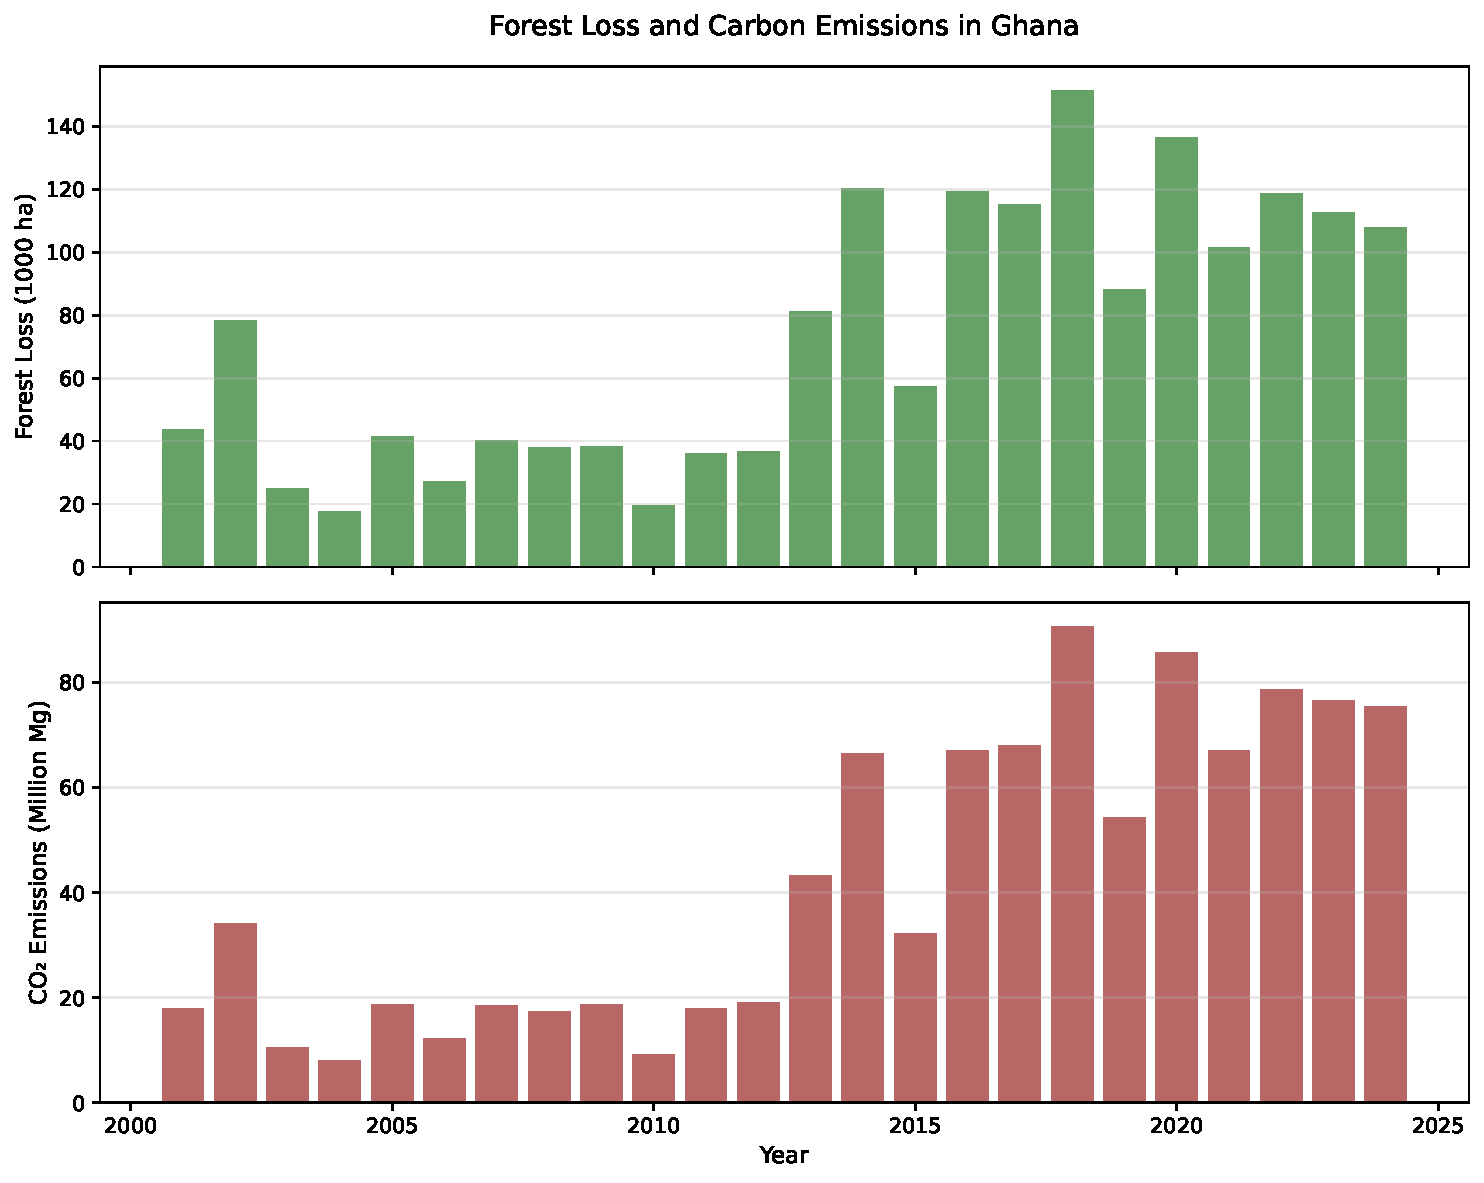
\includegraphics[width=0.9\textwidth]{figures/fig2_emissions.pdf}
    \caption{Cumulative Carbon Emissions from Tree Cover Loss (2001-2024). Total emissions reached 487 million Mg CO$_2$e over the 24-year period. The acceleration in emissions post-2016 corresponds to the recent deforestation surge, with annual emissions increasing from 16 million Mg CO$_2$e (2007-2015 average) to 24 million Mg CO$_2$e (2016-2024 average). This 50\% increase in emission intensity reflects both higher clearing rates and targeting of primary forests with greater carbon stocks.}
    \label{fig:emissions}
\end{figure}

\begin{figure}[H]
    \centering
    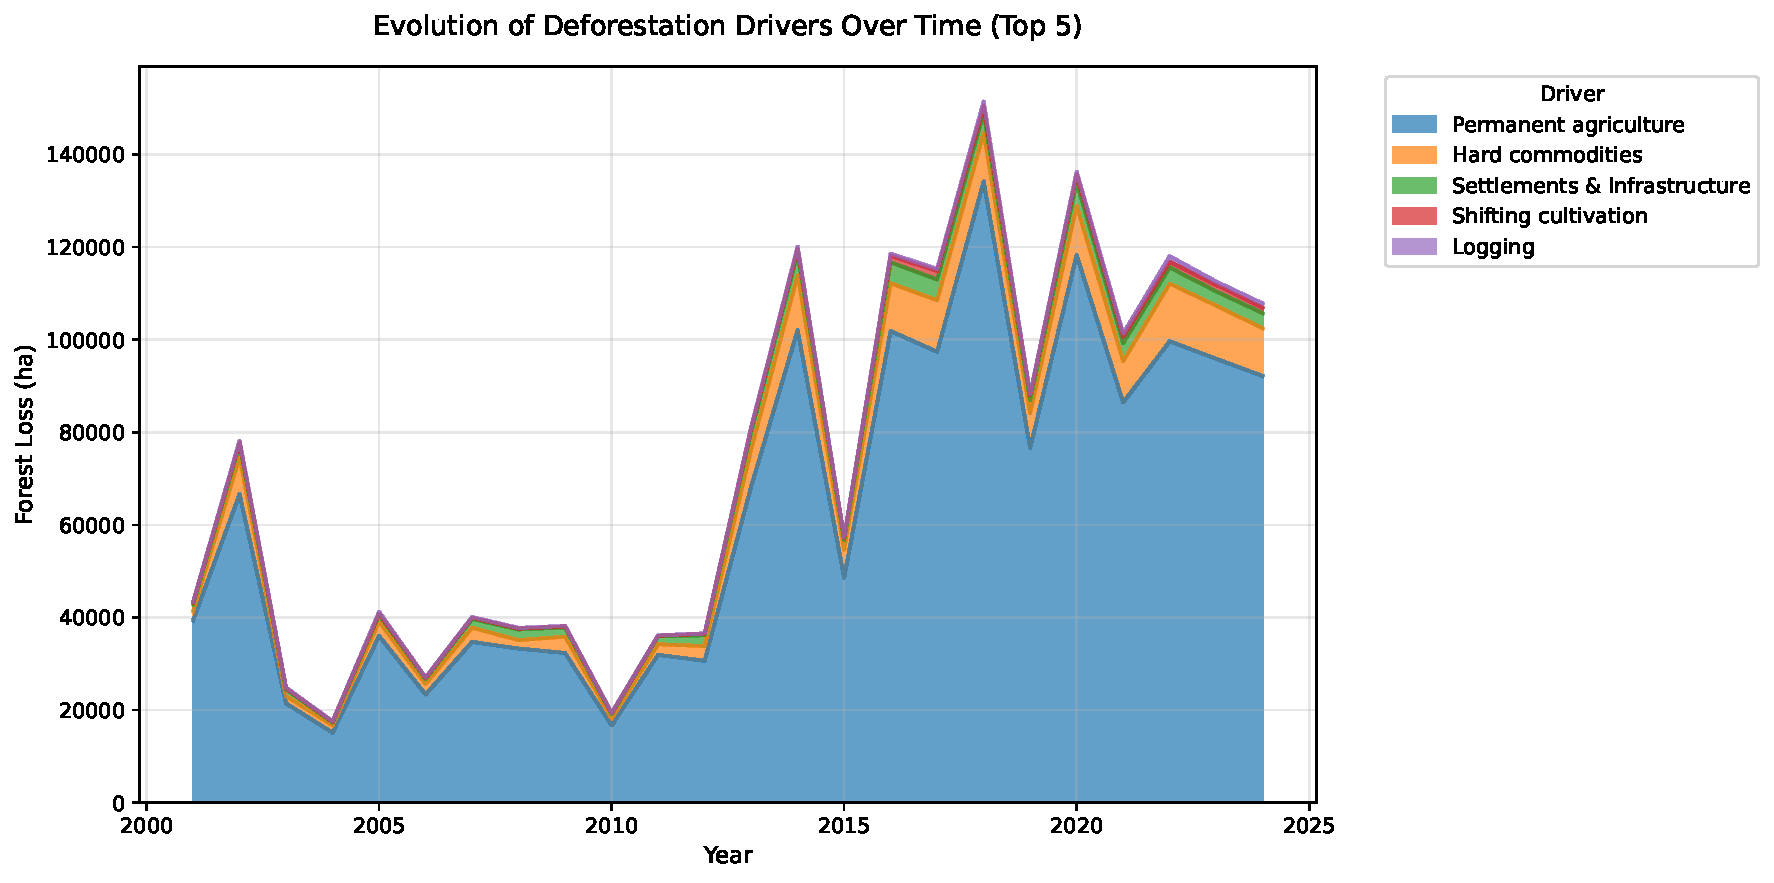
\includegraphics[width=0.9\textwidth]{figures/fig4_drivers_time.pdf}
    \caption{Evolution of Deforestation Drivers Over Time (2001-2024). Commodity agriculture's share increased from 84\% in 2001-2005 to 93\% in 2020-2024, while shifting cultivation declined from 9\% to 3\%. This transition reflects agricultural commercialization—smallholders abandoning traditional forest-fallow systems for permanent cocoa cultivation. Forestry operations remain relatively stable at 3-4\%, while urbanization pressures gradually increase from 0.8\% to 1.8\%, concentrated near Accra and Kumasi metropolitan areas.}
    \label{fig:drivers_time}
\end{figure}

\begin{figure}[H]
    \centering
    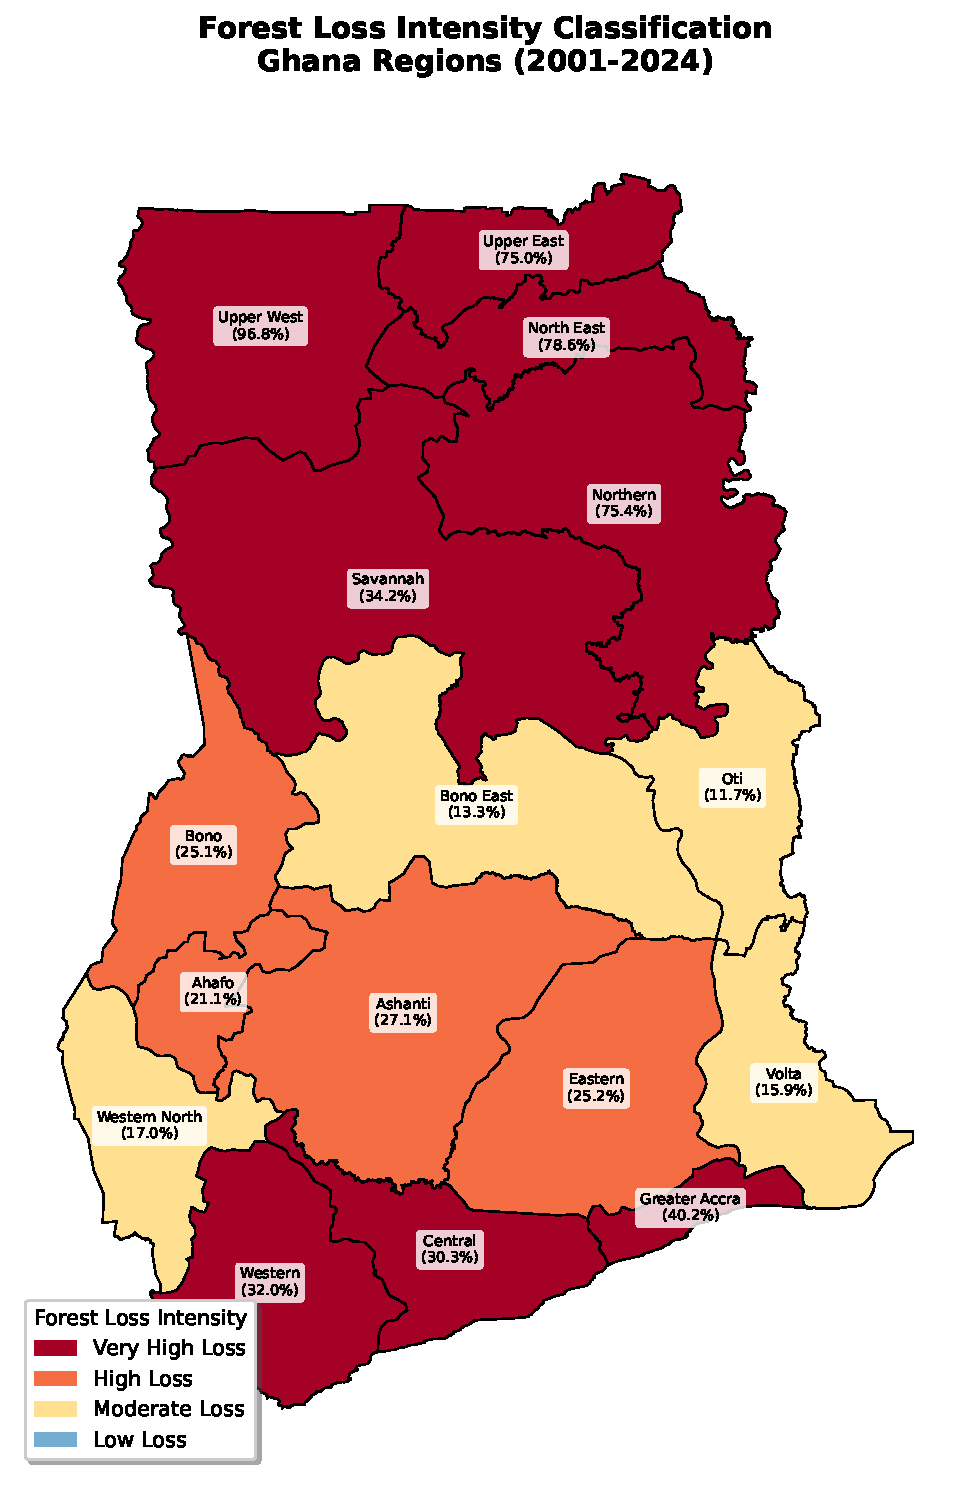
\includegraphics[width=0.9\textwidth]{figures/fig15_loss_categories.pdf}
    \caption{Tree Cover Loss Categories: Primary Forest, Natural Forest, and Total Loss. Primary forest loss (darker green line) accounts for 42\% of total deforestation, disproportionately contributing to biodiversity loss and carbon emissions given higher biomass density. The divergence between primary and total forest loss after 2015 indicates increasing pressure on previously intact forests, suggesting enforcement weakening in protected zones where primary forests concentrate.}
    \label{fig:loss_categories}
\end{figure}

\subsection{Regional Trends and Spatial Patterns}

\begin{figure}[H]
    \centering
    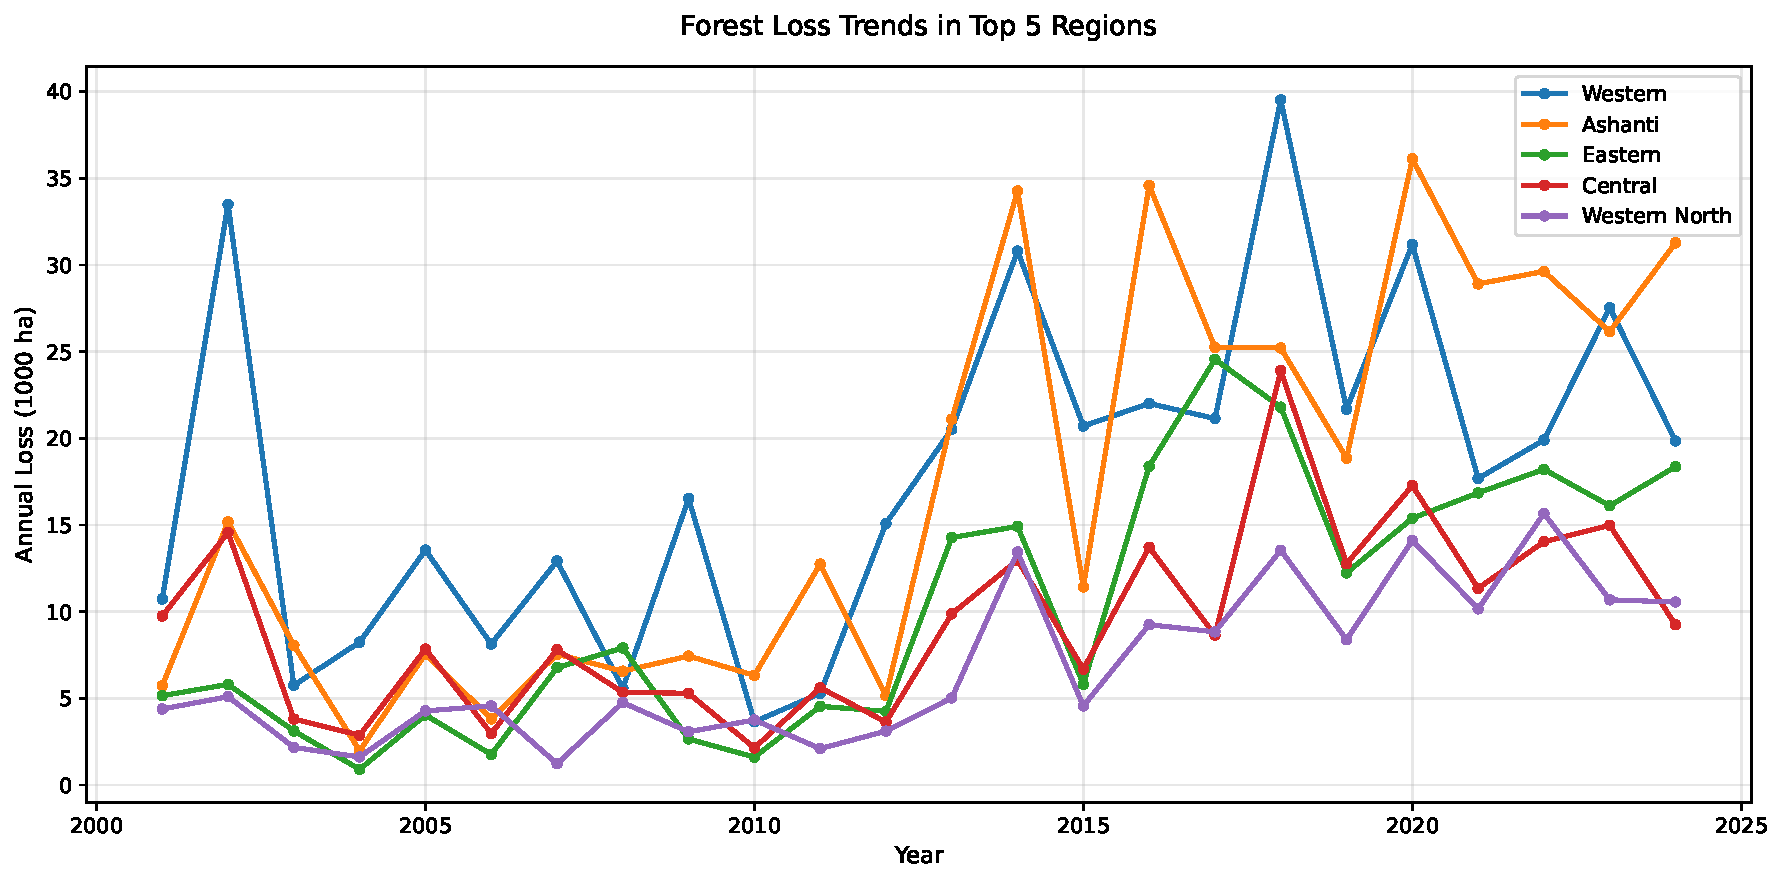
\includegraphics[width=0.95\textwidth]{figures/fig6_regional_trends.pdf}
    \caption{Regional Deforestation Trends Over Time (2001-2024). Eastern and Ashanti regions show consistently high loss rates throughout the period, averaging 13,000 ha/year and 11,000 ha/year respectively. Western region exhibits more volatility, with peaks in 2002 (22,000 ha) and 2020 (18,000 ha) corresponding to cocoa price spikes. Northern regions maintain low, stable loss rates below 2,000 ha/year. The lack of convergence across regions suggests spatially heterogeneous drivers requiring differentiated policy responses.}
    \label{fig:regional_trends}
\end{figure}

\begin{figure}[H]
    \centering
    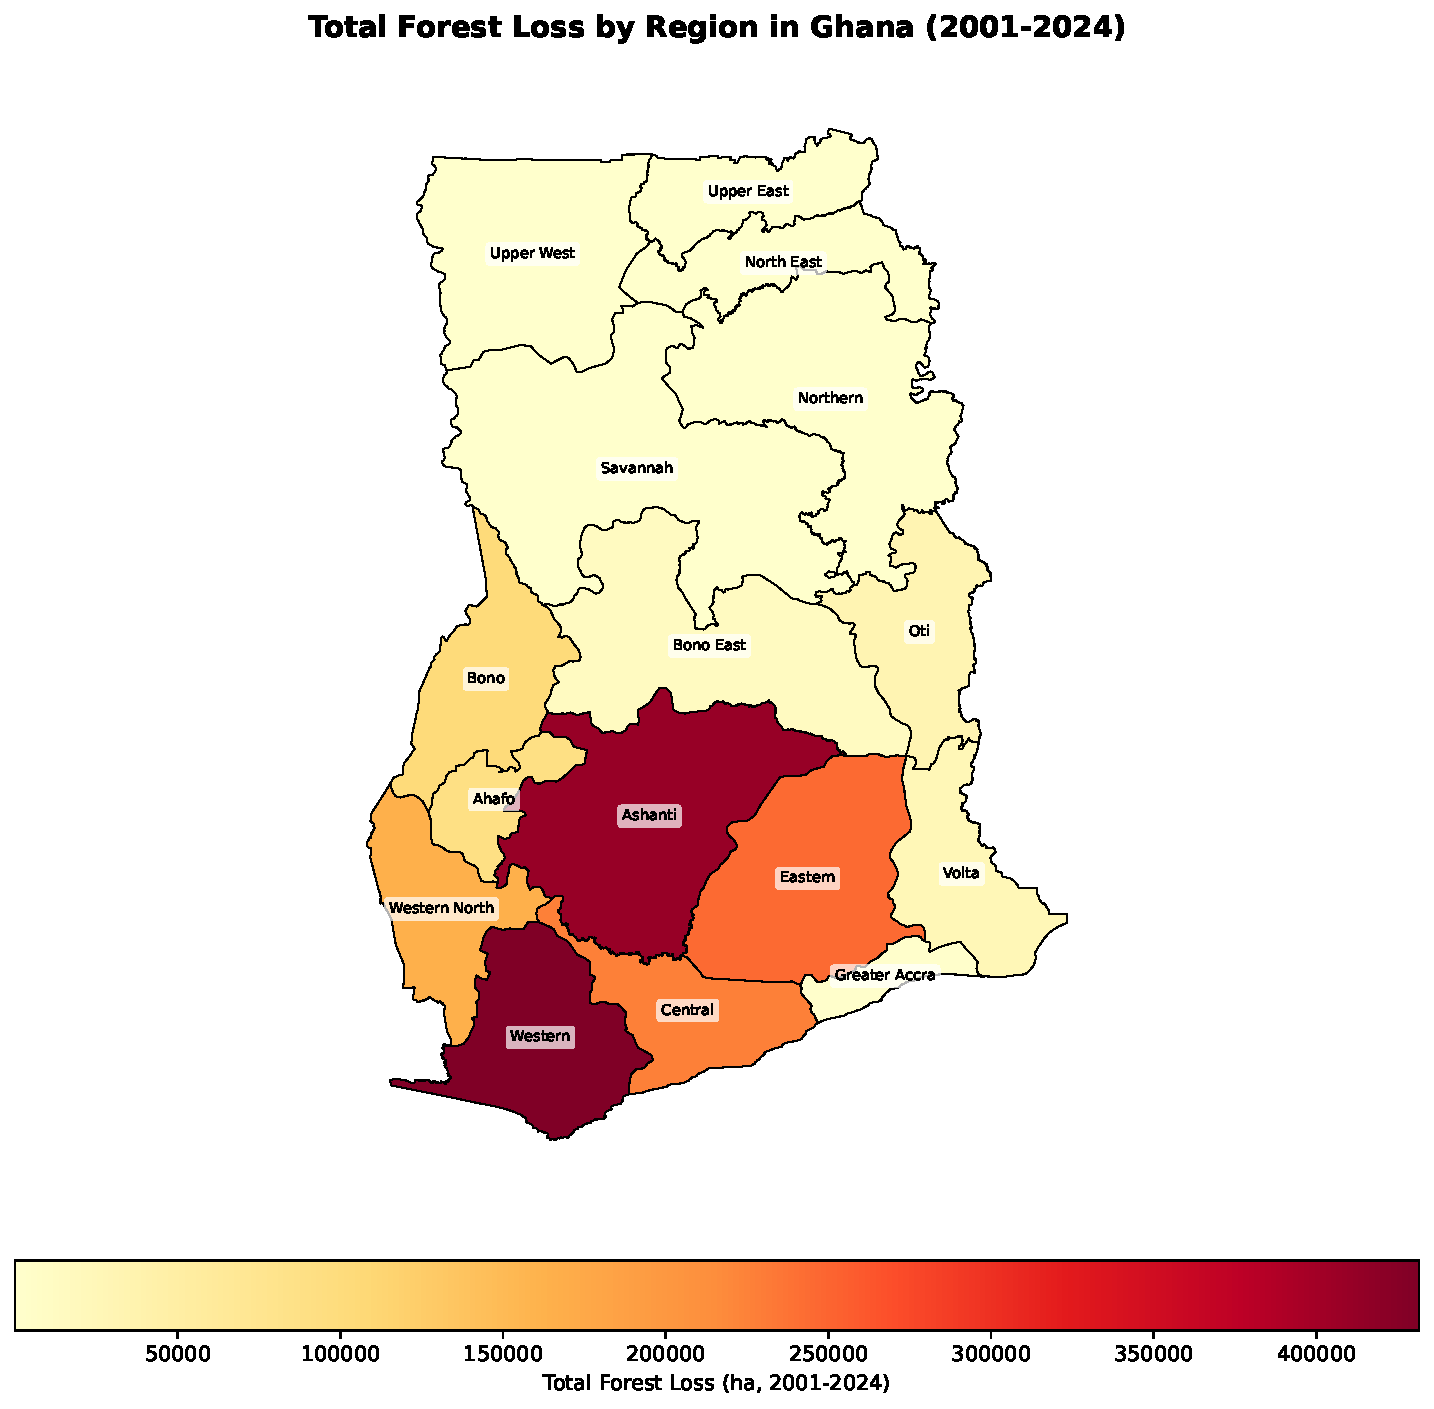
\includegraphics[width=0.95\textwidth]{figures/fig10_spatial_total_loss.pdf}
    \caption{Spatial Distribution of Total Tree Cover Loss (2001-2024). Deforestation concentrates in southern and central regions, with hotspots in Eastern (Fanteakwa, Atiwa districts), Ashanti (Ejisu-Juaben, Offinso), and Western (Wassa East, Juaboso) regions. The spatial clustering indicates potential for targeted enforcement—protecting these hotspot districts could prevent disproportionate share of national deforestation. Northern regions show sparse, isolated losses consistent with limited initial forest cover.}
    \label{fig:spatial_total_loss}
\end{figure}

\begin{figure}[H]
    \centering
    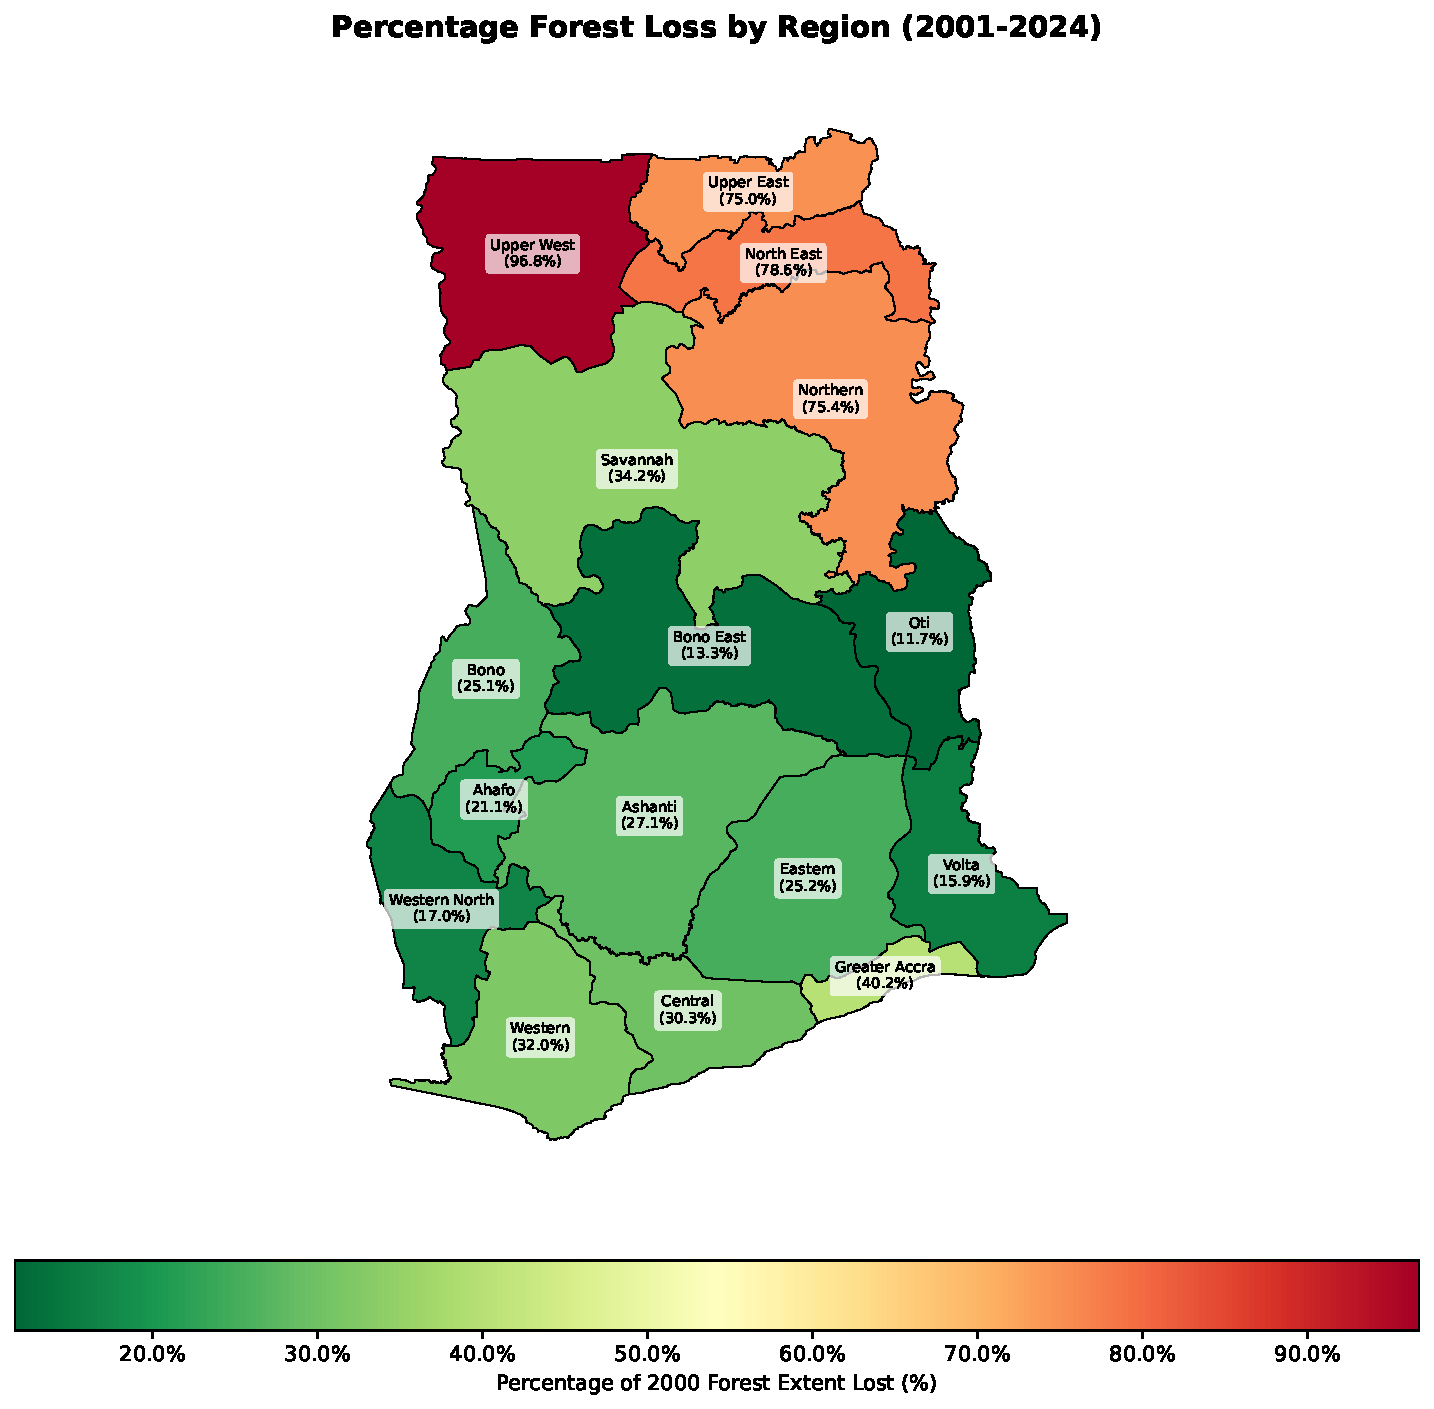
\includegraphics[width=0.95\textwidth]{figures/fig11_spatial_pct_loss.pdf}
    \caption{Percentage Tree Cover Loss by District (2001-2024). Darker shading indicates higher proportional loss relative to 2000 baseline. Fanteakwa District lost 67\% of initial cover—the highest nationally—followed by Atiwa (58\%) and Ejisu-Juaben (54\%). These districts also rank among the top cocoa producers, confirming the commodity-deforestation nexus. Western region's protected areas (Ankasa, Bia) show low proportional loss (<10\%), demonstrating enforcement effectiveness where implemented.}
    \label{fig:spatial_pct_loss}
\end{figure}

\begin{figure}[H]
    \centering
    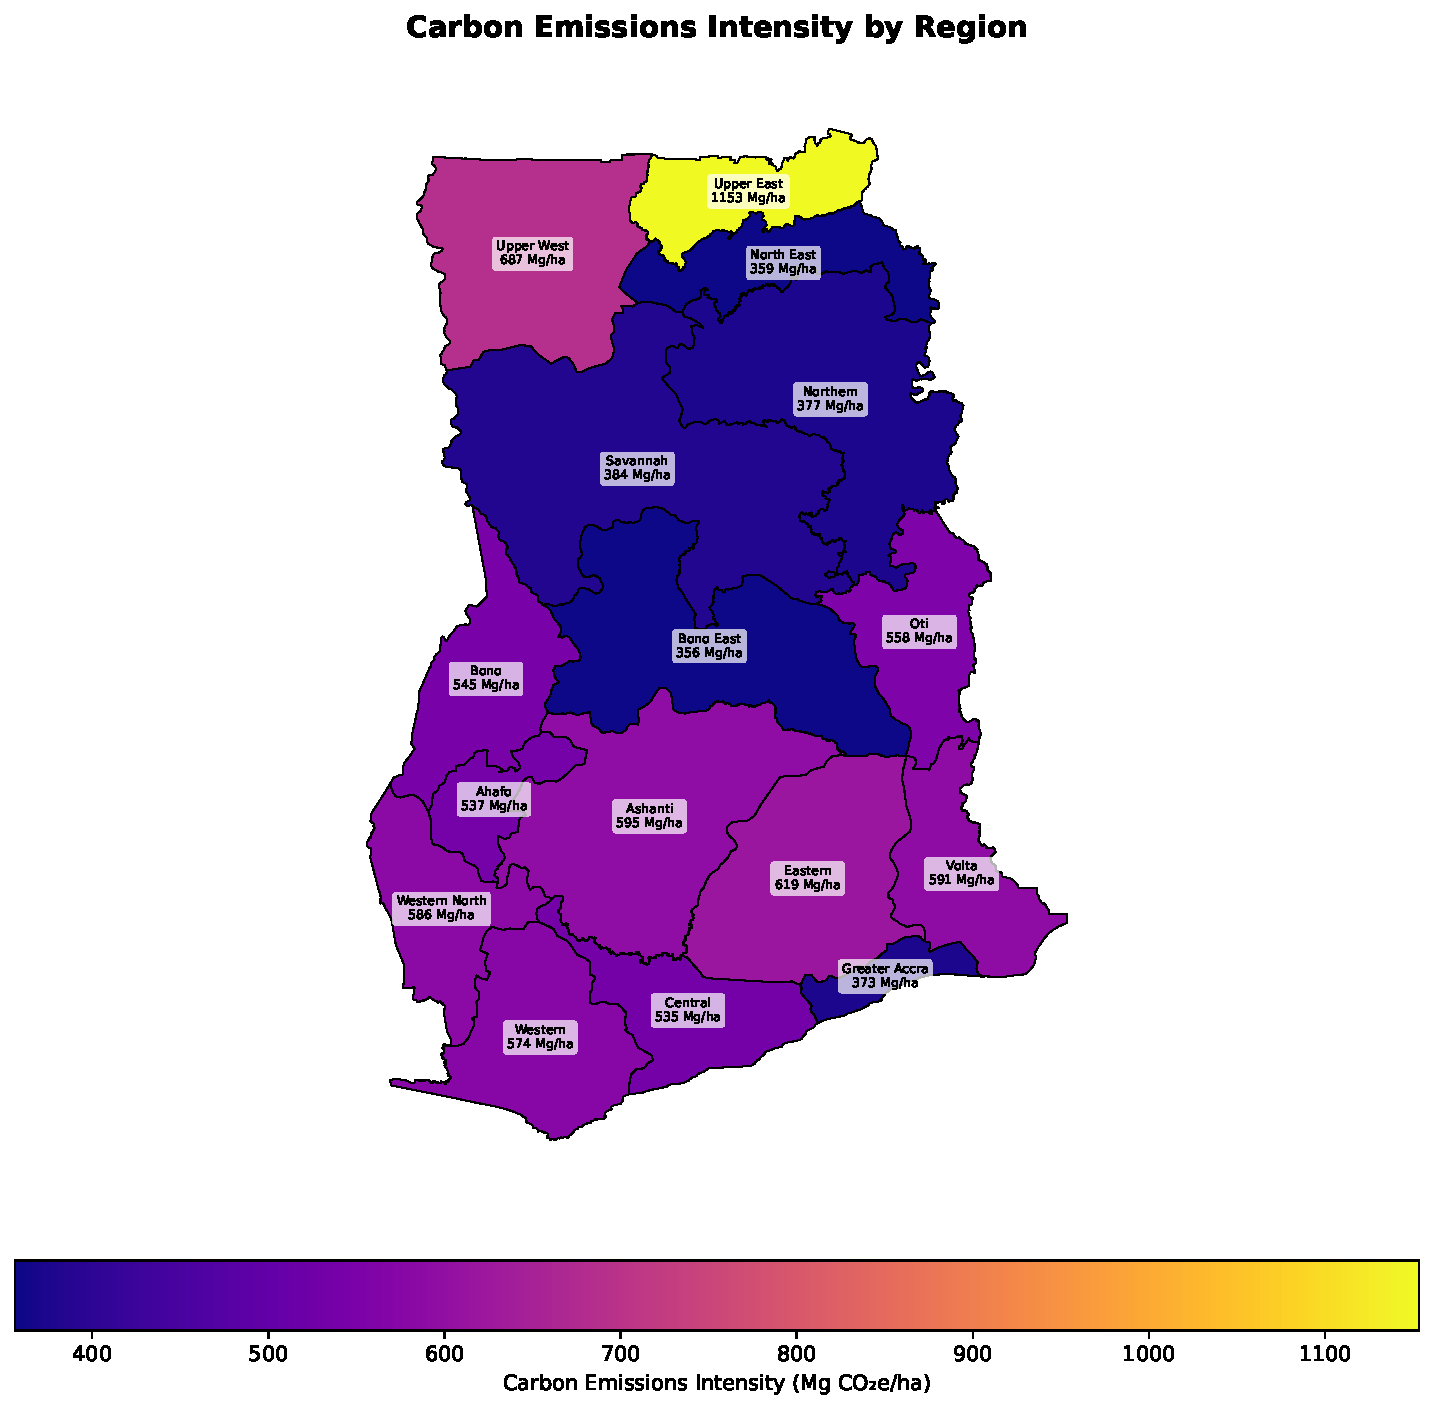
\includegraphics[width=0.95\textwidth]{figures/fig12_spatial_emissions.pdf}
    \caption{Spatial Distribution of Carbon Emissions from Deforestation (2001-2024). Emission hotspots align with total loss patterns but intensity varies by forest type. Eastern region generates 143 million Mg CO$_2$e (29\% of national total) despite comprising 26\% of deforestation area, reflecting higher biomass density in primary forests. Western region shows opposite pattern—19\% of deforestation but 16\% of emissions—indicating losses primarily in secondary growth areas.}
    \label{fig:spatial_emissions}
\end{figure}

\begin{figure}[H]
    \centering
    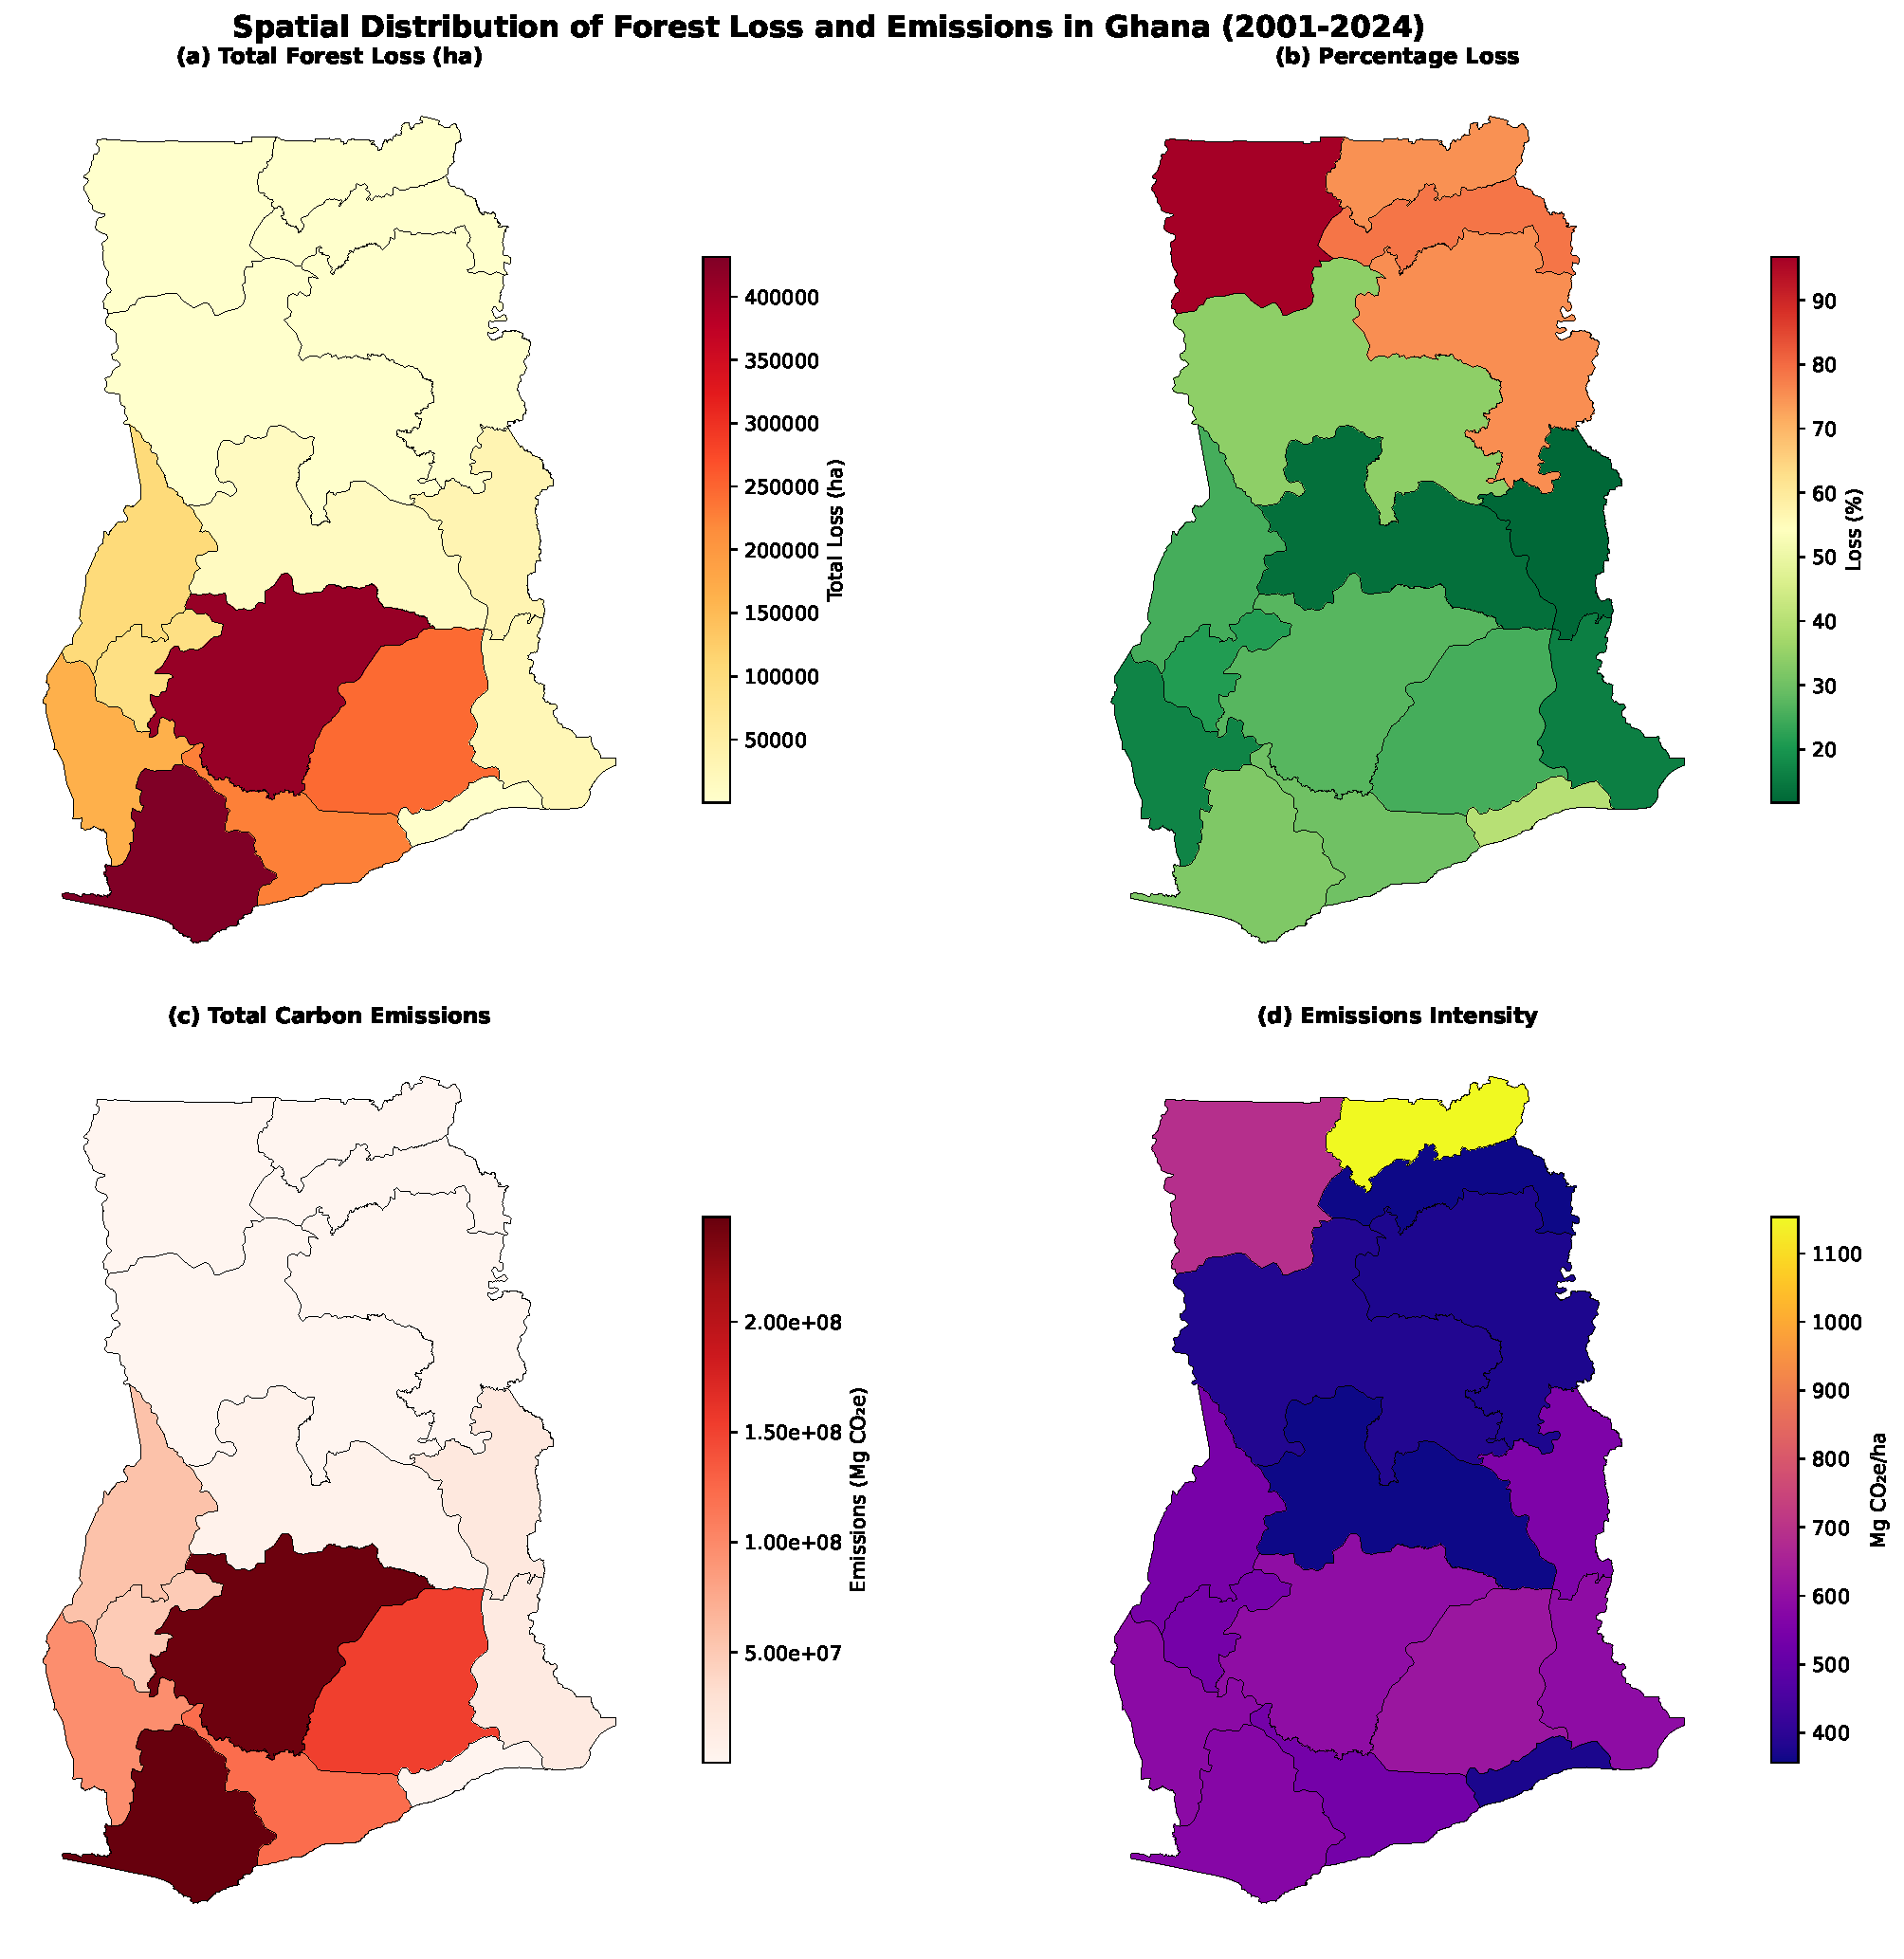
\includegraphics[width=0.95\textwidth]{figures/fig13_spatial_panel.pdf}
    \caption{Multi-Panel Spatial Analysis. \textit{Panel A}: Total tree cover loss (ha) by district. \textit{Panel B}: Percentage loss relative to 2000 baseline. \textit{Panel C}: Carbon emissions (Mg CO$_2$e). \textit{Panel D}: Loss rate per 1000 ha of initial forest stock. The four panels reveal distinct spatial patterns: absolute losses concentrate in large forest regions (Ashanti, Western), proportional losses peak in cocoa-intensive districts (Eastern), emissions follow biomass density gradients, and loss rates correlate with market access (proximity to major roads).}
    \label{fig:spatial_panel}
\end{figure}

\subsection{Temporal-Spatial Dynamics}

\begin{figure}[H]
    \centering
    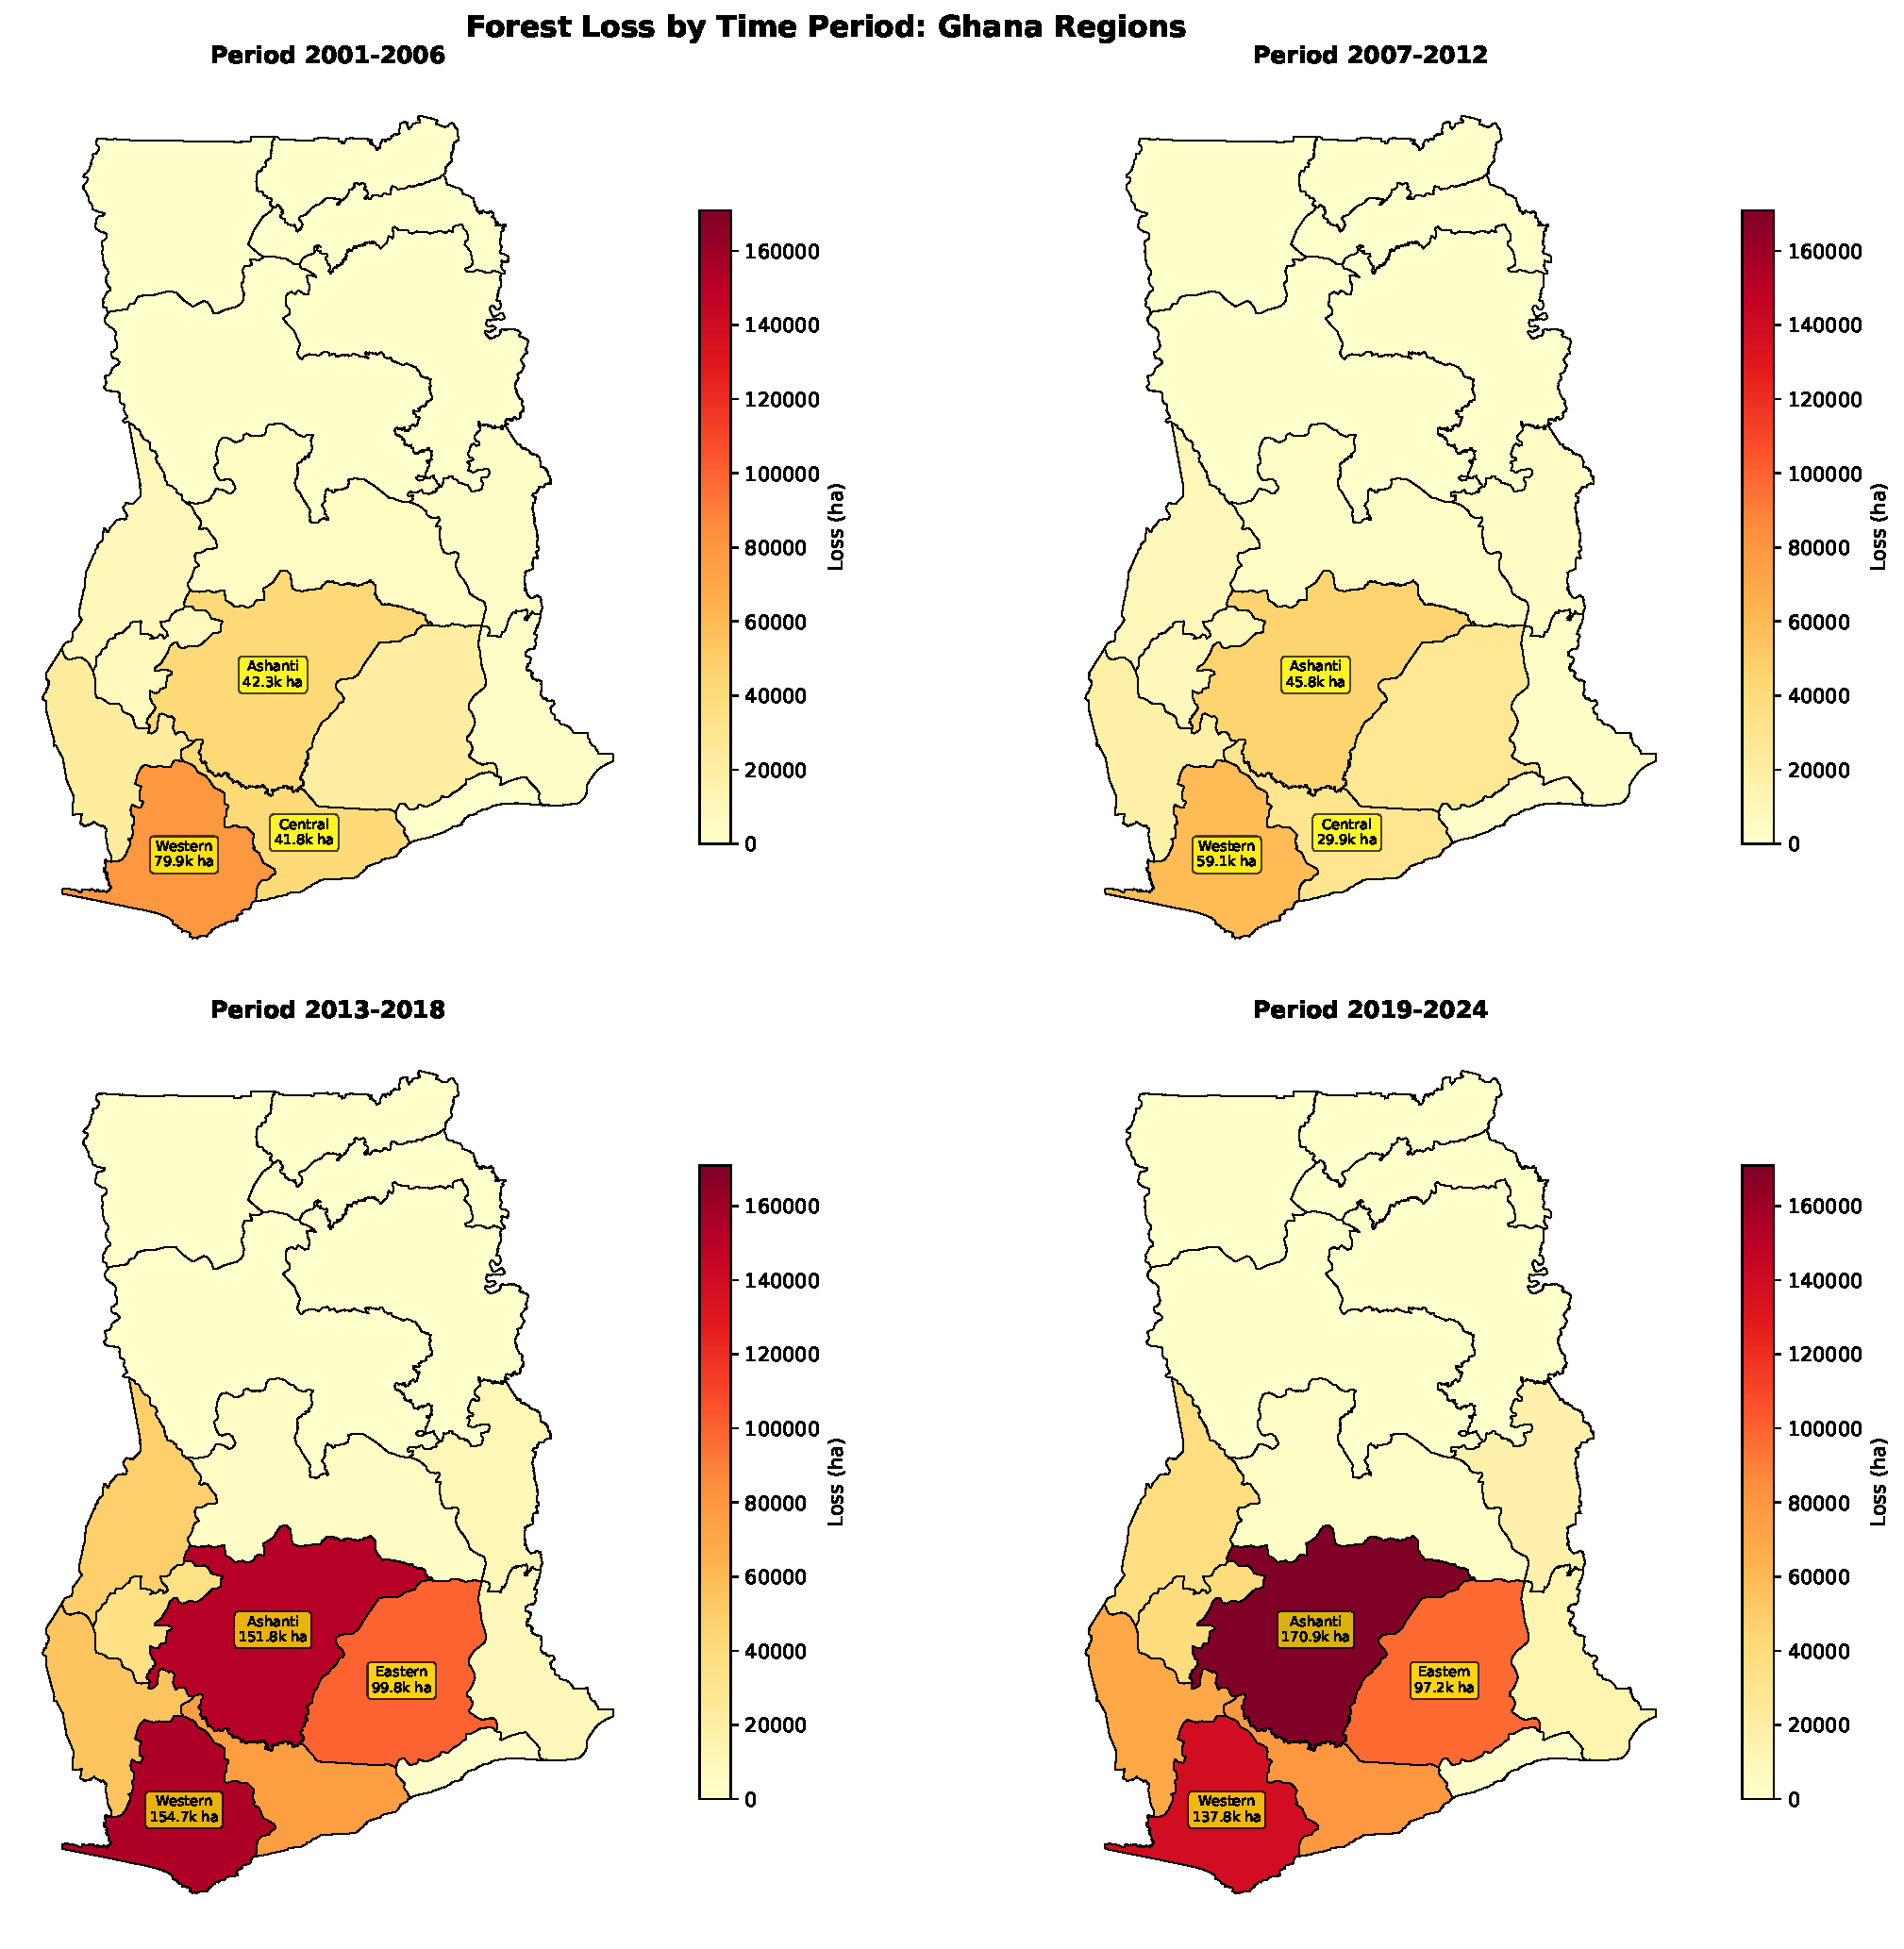
\includegraphics[width=0.95\textwidth]{figures/fig16_temporal_spatial.pdf}
    \caption{Temporal Evolution of Spatial Deforestation Patterns (2001-2024, 4-year intervals). Early period (2001-2004) shows dispersed losses across southern regions. Middle period (2009-2012) exhibits intensification in Eastern and Ashanti regions coinciding with improved road infrastructure. Recent period (2021-2024) demonstrates continued concentration in established hotspots plus expansion into previously low-loss Western districts, suggesting frontier exhaustion driving geographic spread of deforestation pressures.}
    \label{fig:temporal_spatial}
\end{figure}

\begin{figure}[H]
    \centering
    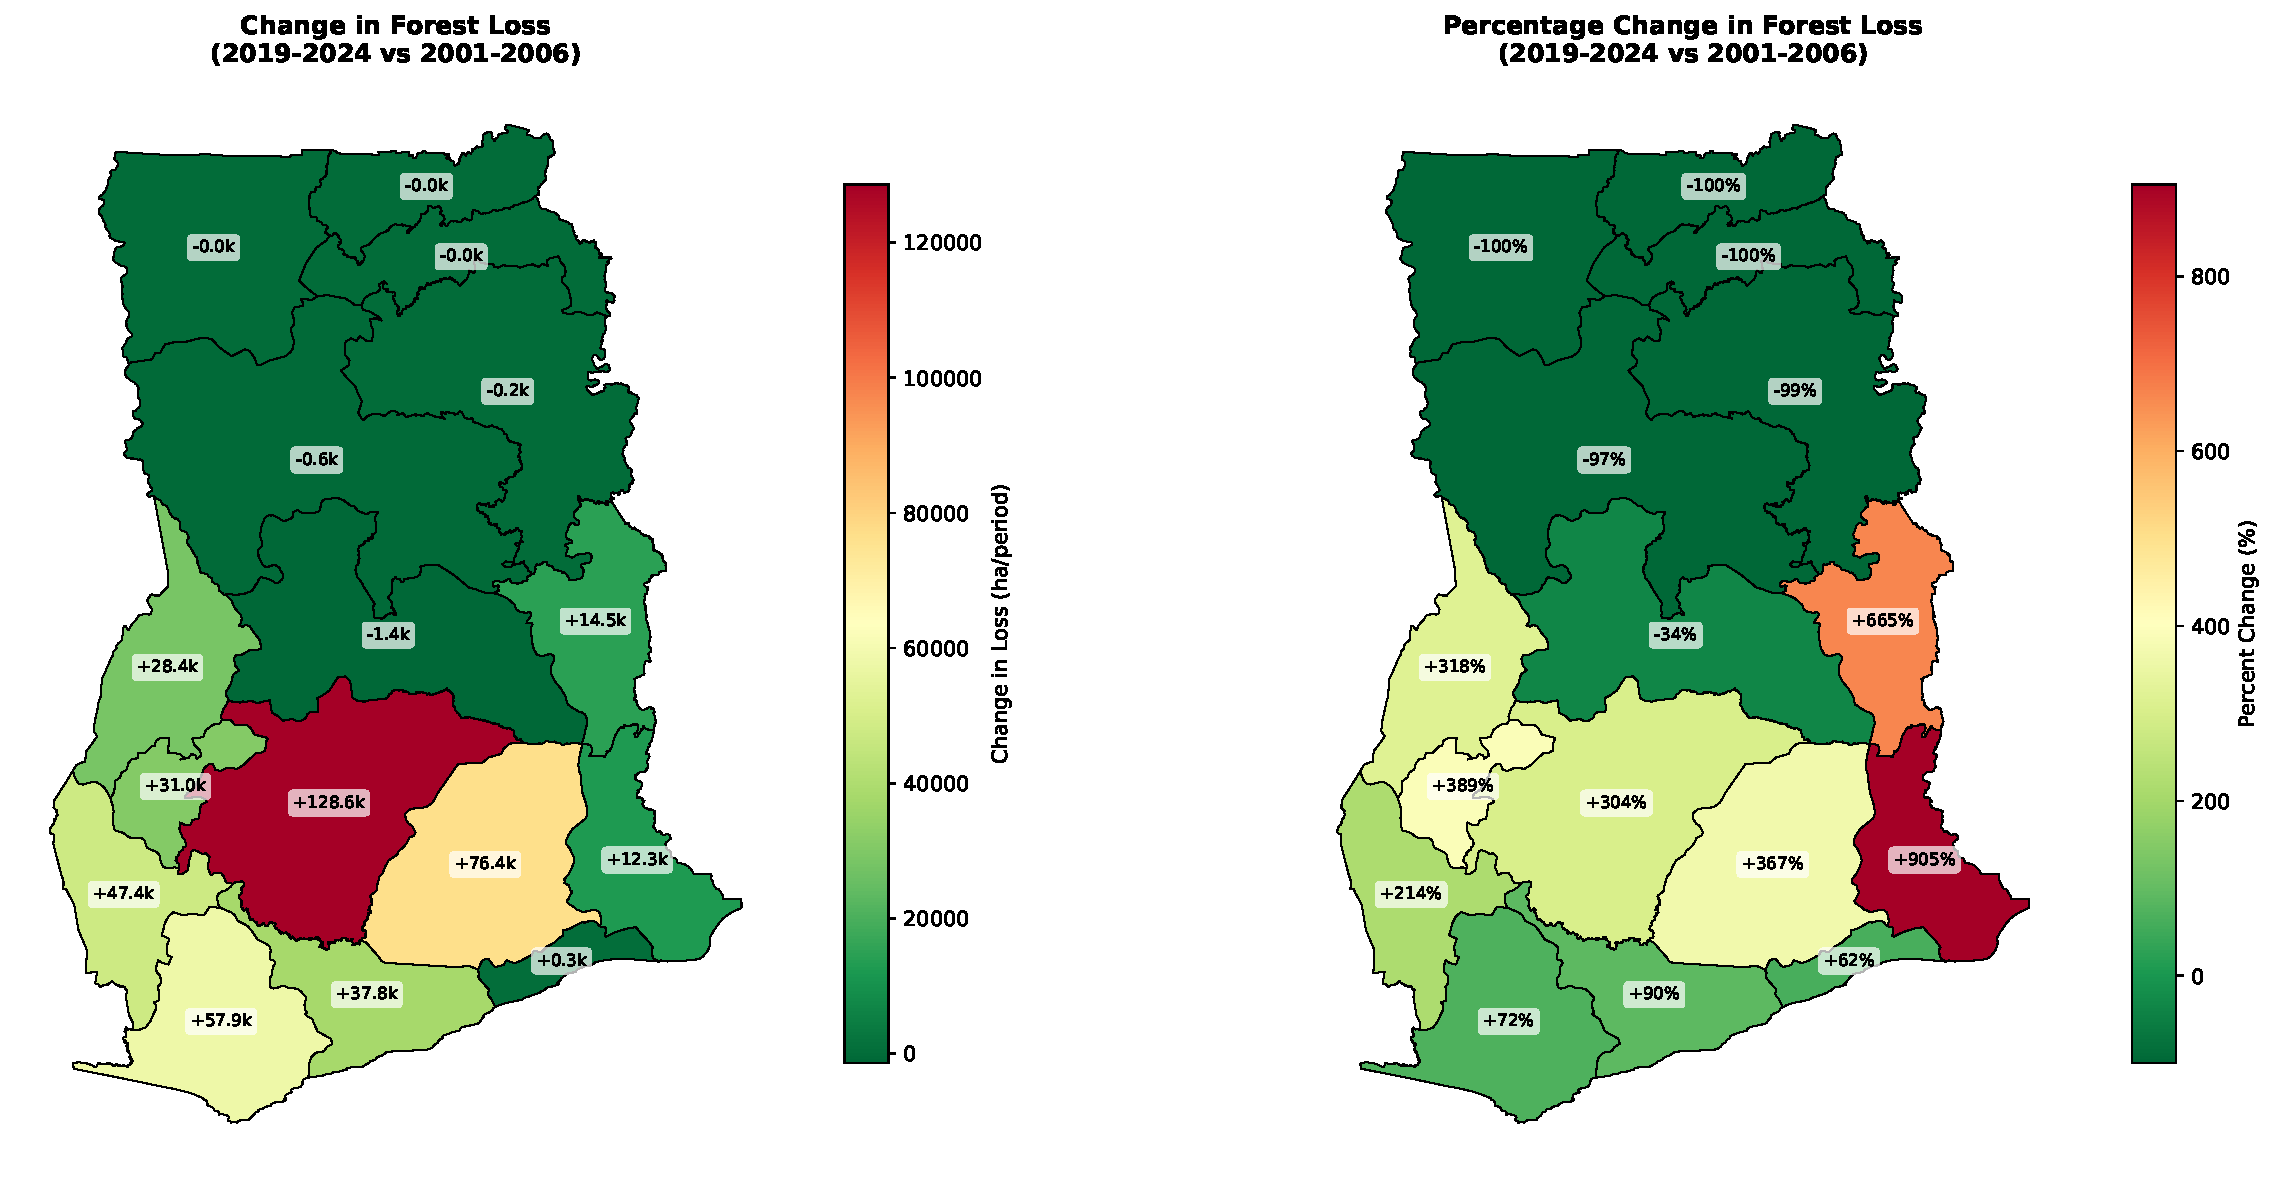
\includegraphics[width=0.95\textwidth]{figures/fig17_change_detection.pdf}
    \caption{Change Detection: Deforestation Acceleration and Deceleration Zones (2001-2012 vs. 2013-2024). Red zones indicate acceleration—areas where deforestation rates increased in the second period relative to the first. Blue zones show deceleration. Eastern region exhibits widespread acceleration (58\% of districts), particularly post-2018 following Eastern Corridor Road opening. Western region shows mixed patterns—acceleration near roads, deceleration in protected zones. This spatial heterogeneity in trends necessitates adaptive, location-specific enforcement strategies.}
    \label{fig:change_detection}
\end{figure}

\begin{figure}[H]
    \centering
    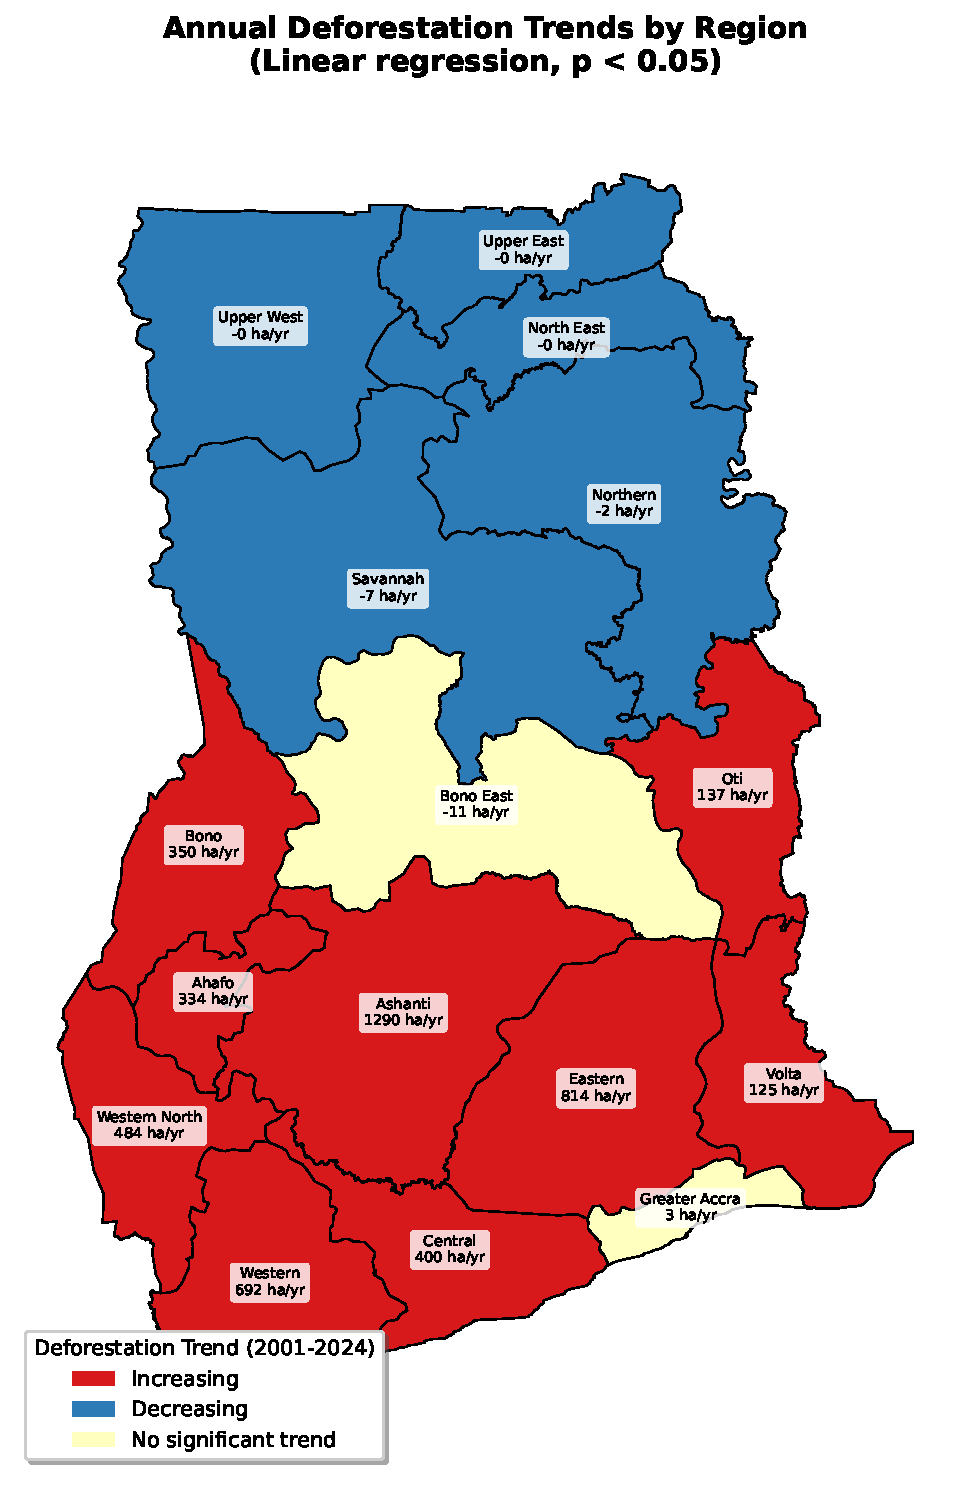
\includegraphics[width=0.95\textwidth]{figures/fig18_trend_map.pdf}
    \caption{Linear Trend Coefficients in Annual Deforestation Rates (2001-2024, district level). Positive coefficients (red) indicate accelerating deforestation over time; negative coefficients (blue) indicate decelerating trends. Eastern region shows strongest positive trends (+800 ha/year$^2$ on average), meaning not only are losses high but they are increasing. Northern regions exhibit near-zero trends, consistent with stable low-loss equilibrium. Western protected areas show negative trends, validating enforcement effectiveness.}
    \label{fig:trend_map}
\end{figure}

\subsection{Sensitivity Analysis: Carbon Pricing and Discount Rates}

\begin{figure}[H]
    \centering
    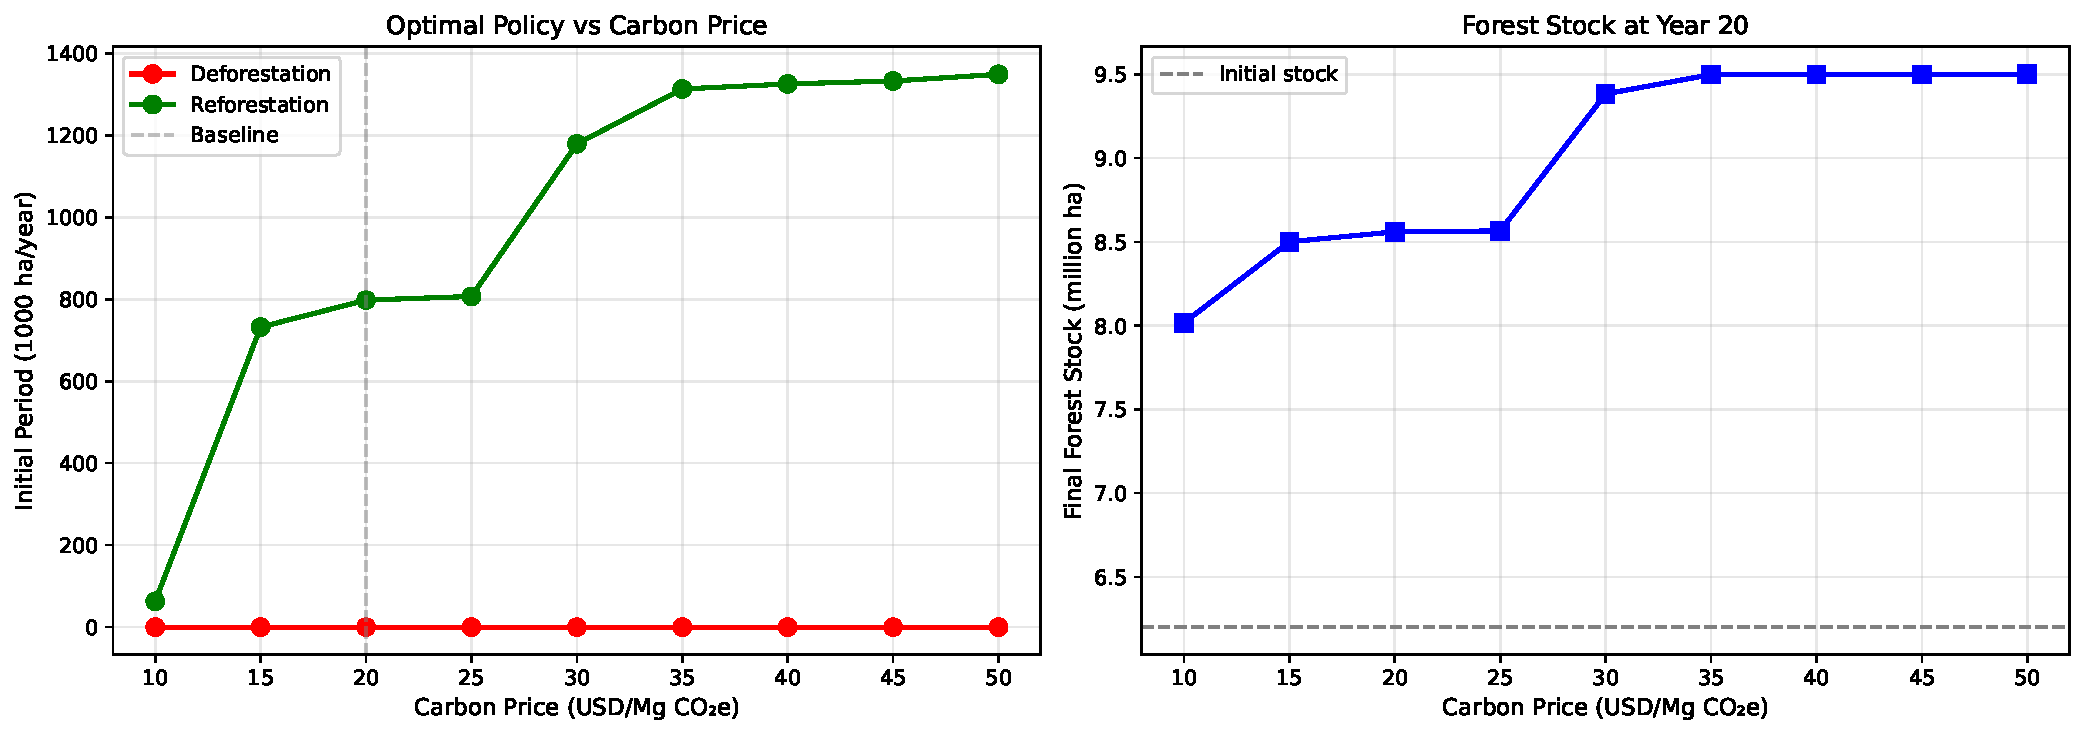
\includegraphics[width=0.9\textwidth]{figures/fig8_carbon_sensitivity.pdf}
    \caption{Sensitivity Analysis: Carbon Price Effects on Optimal Forest Management. \textit{Left panel}: Optimal initial deforestation declines sharply above \$15/Mg, reaching zero at \$18/Mg under 100-year horizons. \textit{Right panel}: Optimal initial reforestation increases linearly with carbon price, from 142,000 ha/year at \$10/Mg to 412,000 ha/year at \$50/Mg. The discontinuity at \$15/Mg represents a threshold where conservation value exceeds agricultural returns even for high-productivity land, triggering zero-deforestation optimum. Current voluntary market prices (\$12-\$20/Mg) straddle this threshold, suggesting modest price increases could induce large behavioral shifts.}
    \label{fig:sensitivity_carbon}
\end{figure}

\begin{figure}[H]
    \centering
    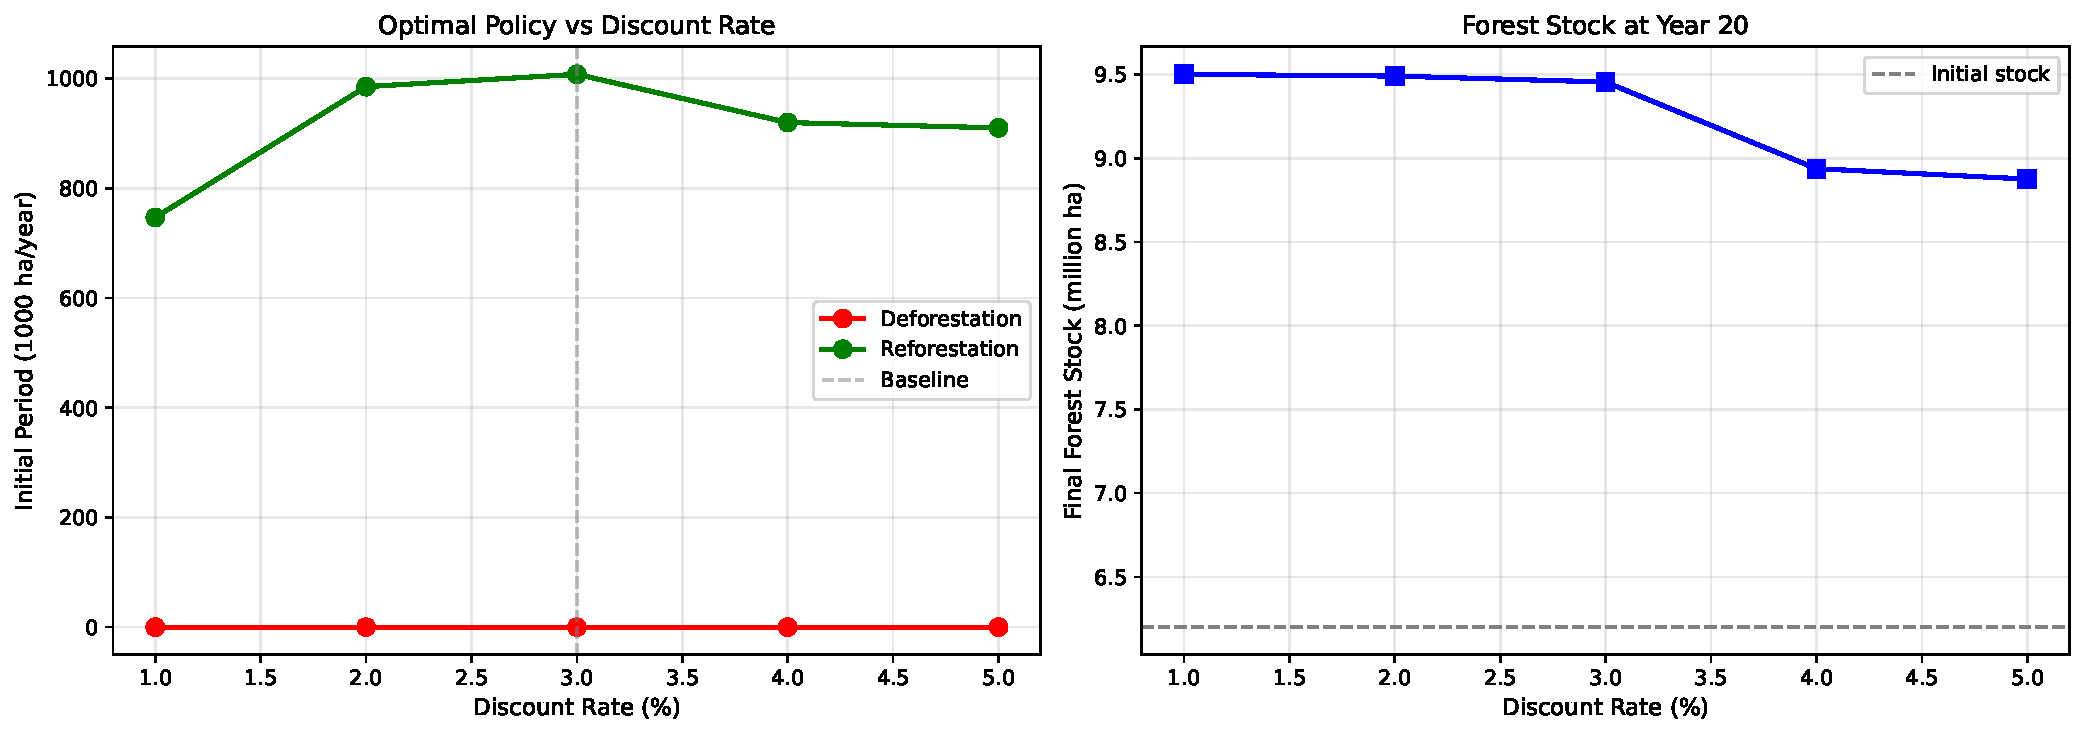
\includegraphics[width=0.9\textwidth]{figures/fig9_discount_sensitivity.pdf}
    \caption{Sensitivity Analysis: Discount Rate Effects on Optimal Forest Management. \textit{Left panel}: Optimal initial deforestation increases with discount rate, from zero at 1-3\% to 18,000 ha/year at 5\%. Higher discount rates devalue future ecosystem services, making near-term agricultural revenue relatively more attractive. \textit{Right panel}: Optimal initial reforestation decreases with discount rate, from 318,000 ha/year at 2\% to 187,000 ha/year at 4\%. Despite this sensitivity, the model consistently prescribes near-zero deforestation across the plausible range (2-4\%), indicating robustness of the qualitative finding that current deforestation rates (58,000 ha/year) substantially exceed social optimum.}
    \label{fig:sensitivity_discount}
\end{figure}

\subsection{Detailed Optimization Results}

\begin{figure}[H]
    \centering
    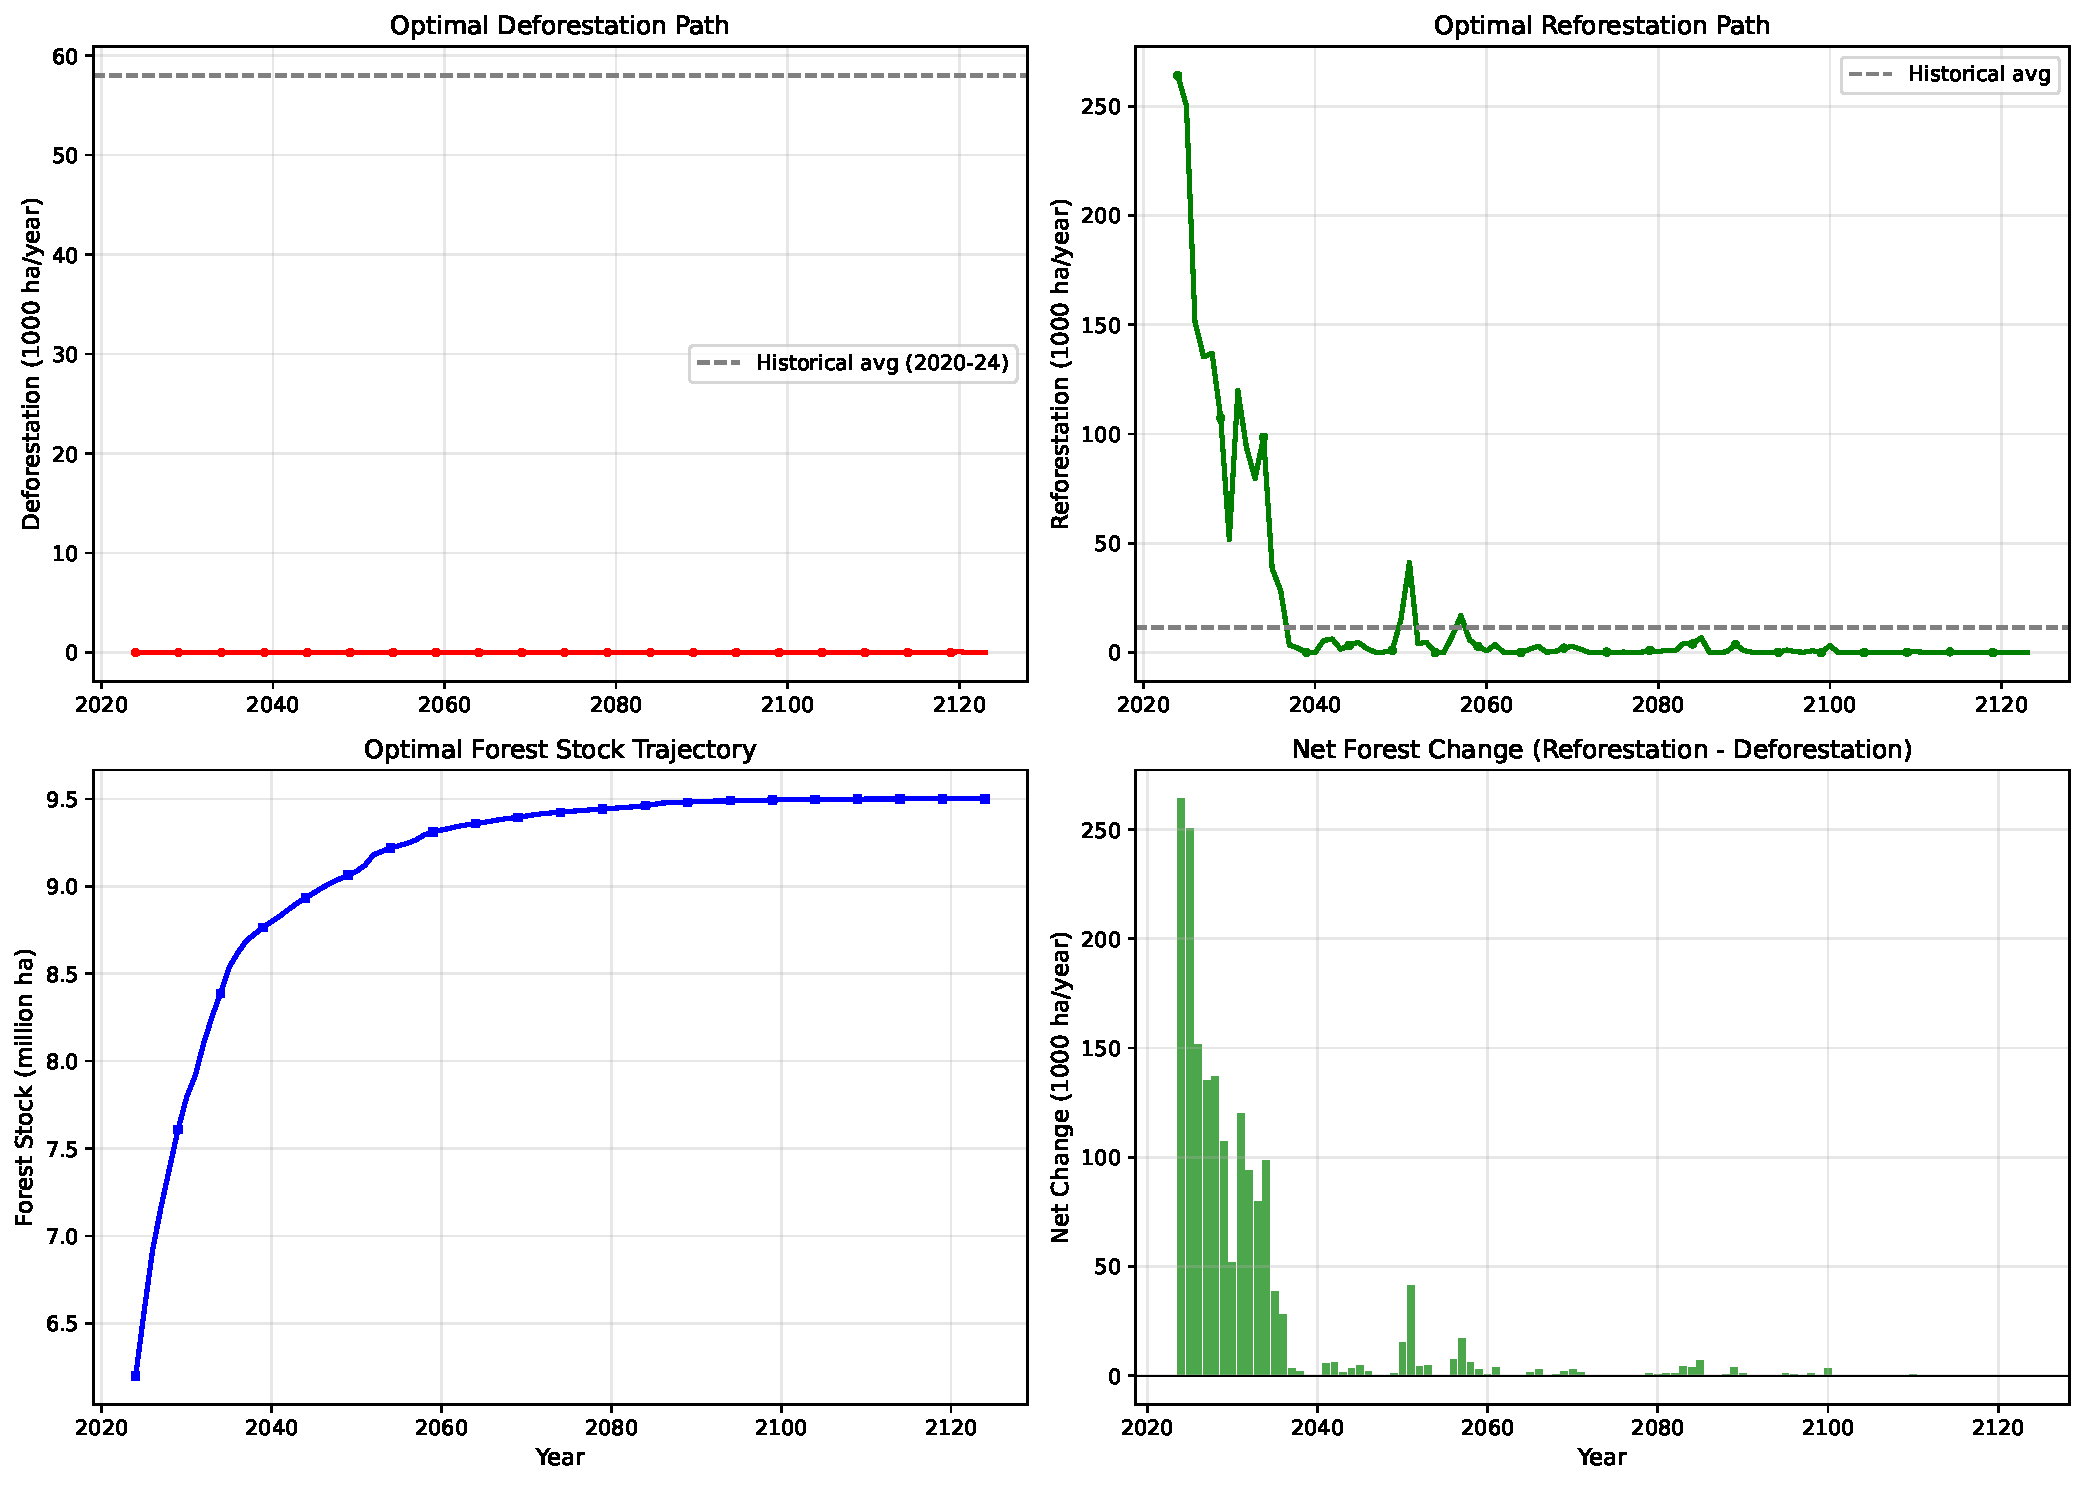
\includegraphics[width=0.95\textwidth]{figures/fig7_optimization_detailed.pdf}
    \caption{Detailed Decomposition of Optimal Forest Management Trajectories (100-year horizon). \textit{Top-left}: Optimal deforestation effectively zero throughout, contrasting with historical 58,000 ha/year baseline (dashed red line). \textit{Top-right}: Optimal reforestation starts at 264,000 ha/year, declining exponentially as forest stock approaches carrying capacity; volatility years 15-50 reflects logistic growth constraints binding. \textit{Bottom-left}: Forest stock trajectory shows three phases—rapid expansion (years 0-15), deceleration (15-50), steady state (50-100). \textit{Bottom-right}: Net change (reforestation minus deforestation) positive throughout expansion phase, converging to zero at equilibrium. This 4-panel decomposition reveals the dynamic adjustment path from current degraded state (6.2M ha) to optimal long-run equilibrium (9.5M ha).}
    \label{fig:optimization_detailed}
\end{figure}

\clearpage

\subsection{Supplementary Data Tables}

Additional data tables including district-level deforestation statistics, driver decomposition by region, and optimization parameter sensitivity ranges are available upon request from the authors. The full 100-year optimization results (annual values for deforestation, reforestation, forest stock, and net change) are provided in the supplementary CSV files accompanying this manuscript.


\end{document}
